\documentclass[a4paper, 11pt]{article}

\usepackage[utf8]{inputenc}
\usepackage{verbatim}
\usepackage{moreverb}
\usepackage[english]{babel}
\usepackage[T1]{fontenc}
\usepackage{lmodern}
\usepackage{graphicx}
\usepackage{fancyhdr}
\usepackage{listings} 
\usepackage{lastpage}
\usepackage[top=3cm, bottom=3cm, left=2cm, right=2cm]{geometry}
\usepackage{color}
\usepackage{xcolor}
\usepackage{epstopdf} 
%font change
\renewcommand{\familydefault}{\sfdefault}

\newcommand{\HRule}{\rule{\linewidth}{0.3mm}}
\newcommand{\nl}{\\[0.1cm]}
\newcommand{\s}{\vspace{0.3cm}}
\newcommand{\emptypage}{\newpage \thispagestyle{empty} \mbox{}\newpage}
\newcommand{\smore}{\vspace{0.6cm}}
\newcommand{\emphasis}[1]{\textbf{#1}}

\usepackage{caption}
\DeclareCaptionFont{white}{\color{white}}
\DeclareCaptionFormat{listing}{\colorbox{gray}{\parbox{\textwidth}{#1#2#3}}}
\captionsetup[lstlisting]{format=listing,labelfont=white,textfont=white}

\lstset{frame=single,basicstyle=\ttfamily}

\lstdefinelanguage{popc}{%
   morekeywords={%
   %od
      od, url, power, @, 100, 80, machine, POPString, search
  },
  sensitive=true,
  morestring=[b]',
}

\addto\captionsenglish{%
  \renewcommand{\listfigurename}{}%
	\renewcommand\refname{}
}

%Header and footer 
\pagestyle{fancy}
\fancyhead{}
\fancyfoot{}

%Header definition
\renewcommand{\headrulewidth}{0.5pt}
\lhead{POP-Java : User and Installation Manual}

%Footer definition
\renewcommand{\footrulewidth}{0.5pt}
\cfoot{\today}
\lfoot{Clément Valentin, Beat Wolf}
\rfoot{Page \thepage ~on \pageref{LastPage}}

%remove indent for paragraph
\parindent0ex 

%\setlength{\parskip2ex}

\begin{document}

% TITLE
% TITLE INFORMATION

\begin{titlepage}
 
\begin{center}

\includegraphics[scale=0.5]{eif_logo.png}


\includegraphics[scale=0.2]{popjava_official.png}\\[1.5cm]


\HRule \\[1cm]
{ \huge \bfseries Parallel Object Programming Java\\[0.3cm]
User and Installation Manual}\\[0.5cm]
 \begin{center}
 Software version : 1.0\\
 Manual version : 1.0
 \end{center}
\HRule \\[2cm]
 
% Author and supervisor
\begin{minipage}{0.4\textwidth}
\begin{flushleft} \large
\textbf{Author:}\\
Valentin Clément\\[0.3cm]
\textbf{Expert:}\\
Christian Senn
\end{flushleft}
\end{minipage}
\begin{minipage}{0.4\textwidth}
\begin{flushright} \large
\textbf{Supervisors:} \\
Dr. Pierre Kuonen\\
Dr. Van Hoai Tran\\
Pr. François Kilchoer\\
Jean-François Roche
\end{flushright}
\end{minipage}
 
\vfill
  
\end{center}
 
\end{titlepage}


%\emptypage
% CONTENTS
\tableofcontents
\pagebreak

\section{Remarks}
This document is part of the bachelor thesis project named "POP-Java" written by Valentin Clément in 2010.

% INTRODUCTION
%\emptypage
\pagebreak
\section{Introduction and background}
\subsection{Introduction}
Programming large heterogeneous distributed environments such as GRID or P2P
infrastructures is a challenging task. This statement remains true even if
we consider researches that have focused on enabling these types of
infrastructures for scientific computing such as resource management and
discovery \cite{Foster97, Grimshaw99, Czajkowski98}, service architecture
\cite{Foster02}, security \cite{Welch03} and data management
\cite{Allcock02, Stockinger01}.
Efforts to port traditional programming tools such as MPI
\cite{Foster98:2, Roy00, Karonis03} or BSP \cite{Tong03, Williams00},
also had some success. These tools allow programmers to run their existing
parallel applications on large heterogeneous distributed environments. However,
efficient exploitation of performance regarding the heterogeneity still
needs to be manually controlled and tuned by programmers.\s

POP-C++ and POP-Java are implementations of the POP (\emphasis{P}arallel \emphasis{O}bject
\emphasis{P}rograming) model first introduced by Dr. Tuan Anh Nguyen in
his PhD thesis \cite{Nguyen04}. POP-C++ is an extension of the C++ programming language\cite{Nguyen07} and POP-Java is an extension of the Java programming language\cite{popjava_tech}. The POP model is based on the very simple
idea that objects are suitable structures to distribute data and executable
codes over heterogeneous distributed hardware and to make them interact
between each other.

Inspired by CORBA \cite{corba26} and C++, the POP-C++ programming
language extends C++ by adding a new type of \emphasis{parallel object},
allowing to run C++ objects in distributed environments. With POP-C++,
programming efficients distributed applications is as simple as writing
a C++ programs. The POP-Java programming language extends Java and implements the same mechanisms as POP-C++.

\subsection{The POP model}
The POP model extends the traditional object oriented programming model
by adding the minimum necessary functionality to allow for an easy development
of coarse grain distributed high performance applications.
When the object oriented paradigm has unified the concept of module and type to
create the new concept of \emphasis{class}, the POP model unifies the concept
of class with the concept of \emphasis{task} (or \emphasis{process}). This
is realized by adding to traditional sequential classes a new type of class:
\emphasis{the parallel class}. By instantiating parallel classes we are able
to create a new category of objects we will call \emphasis{parallel objects}
in the rest of this document.\s

Parallel objects are objects that can be remotely executed. They coexist and
cooperate with traditional sequential objects during the application execution.
Parallel objects keep advantages of object-orientation such as data
encapsulation, inheritance and polymorphism and adds new properties to
objects such as:

\begin{itemize}
	\item Distributed shareable objects
	\item Dynamic and transparent object allocation
	\item Various method invocation semantics
\end{itemize}

\subsection{System overview}
Although the POP-C++ programming system focuses on an object-oriented
programming model, it also includes a runtime system which provides the necessary services to run POP-C++ and POP-Java applications over distributed environments. \s

An overview of the POP system (Both POP-C++ and POP-Java) architecture is illustrated in figure[\ref{fig:popsystem}]. In POP-Java, only the programming system is implemented and the runtime system is the same as the one used in POP-C++.


\begin{figure}[ht]
	\caption{POP system architecture}
  	\centering
  	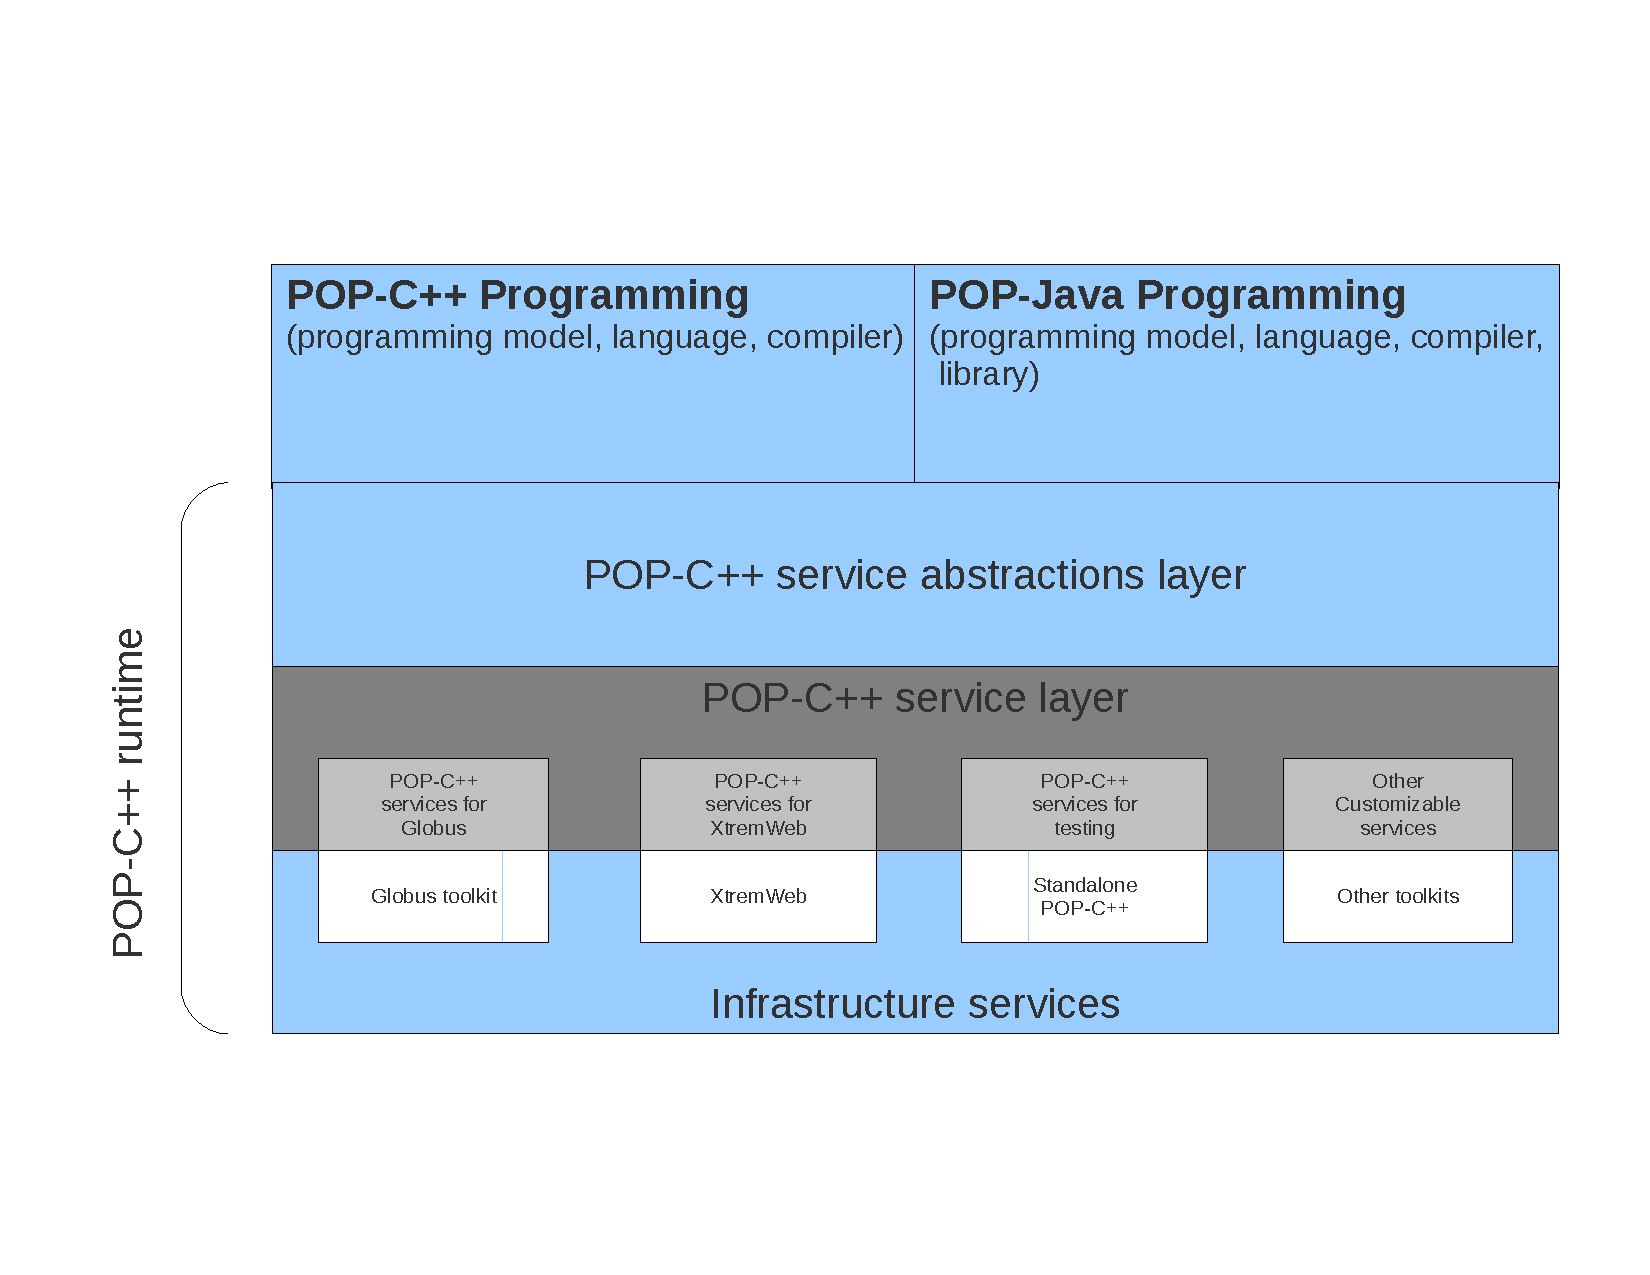
\includegraphics[scale=0.5]{architecture.pdf}
	\label{fig:popsystem}
\end{figure}


The POP-C++ runtime system consists of three layers: the service layer,
the POP-C++ service abstractions layer, and the programming layer. The
service layer is built to interface with lower level toolkits (e.g.
Globus) and the operating system. The essential service abstraction layer
provides an abstract interface for the programming layer. On top of the
architecture is the programming layer, which provides necessary support
for developing distributed object-oriented applications. More details of
the POP-C++ runtime layers are given in a separate document \cite{Nguyen04}.

\subsection{Structure of this manual}
This manual has 8 chapters, including this introduction. The next chapter (chapter \ref{popmodel}) explains the POP model. The chapter \ref{dev} describes the POP-Java application development process. The chapter \ref{compileandrun} explains the compilation and the launch process of a POP-Java application. The chapter \ref{mixed} aims to describe and explain how to use of POP-C++ and POP-Java together in a same application. The chapter \ref{plugin} describes the POP-Java plugin system. The chapter \ref{install} guides the user trough the installation process. Finally, the chapter \ref{trouble} gives some hints to solve the main problems that can occurs with a POP-Java application.



% POP
\pagebreak
\section{Parallel Object Model}
\label{popmodel}
\subsection{Introduction}
Object-oriented programming provides high level abstractions for software
engineering. In addition, the nature of objects makes them ideal
structures to distribute data and executable codes over heterogeneous
distributed hardware and to make them interact between each other.
Nevertheless, two questions remain:

\begin{itemize}

\item Question 1: which objects should run remotely?

\item Question 2: where does each remote object live?

\end{itemize}

The answers, of course, depend on what these objects do and how
they interact with each other and with the outside world. In other
words, we need to know the communication and the computation
requirements of objects. The parallel object model presented in this
chapter provides an object-oriented approach for requirement-driven high
performance applications in a distributed heterogeneous environment.


\subsection{Parallel Object Model}
POP stands for {\it Parallel Object Programming}, and POP parallel objects are
generalizations of traditional sequential objects. POP-Java is an
extension of Java that implements the POP model. POP-Java instantiates
parallel objects transparently and dynamically, assigning suitable
resources to objects. POP-Java also offers various mechanisms to specify
different ways to do method invocations. Parallel objects have all the properties
of traditional objects plus the following ones:

\begin{itemize}

\item Parallel objects are shareable. References to parallel objects can
       be passed to any other parallel object. This property is described in section \ref{shareable}.

\item Syntactically, invocations on parallel objects are identical to
       invocations on traditional sequential objects. However, parallel
       objects support various method invocation semantics: synchronous
       or asynchronous, and sequential, mutex or concurrent. These
       semantics are explained in section \ref{semantic}.

\item Parallel objects can be located on remote resources in separate
       address spaces. Parallel objects allocations are transparent to
       the programmer. The object allocation is presented in section
       \ref{allocation}.

\item Each parallel object has the ability to dynamically describe its
       resource requirement during its lifetime. This feature is
       discussed in detail in section \ref{requirement}

\end{itemize}

As for traditional objects, parallel objects are active only when they execute
a method (non active object semantic). Therefore, communication between
parallel objects are realized thank to remote methods invocation.


\pagebreak
\subsection{Shareable Parallel Objects}
\label{shareable}
Parallel objects are shareable. This means that the reference of a
parallel object can be shared by several other parallel objects.
Sharing references of parallel objects are useful in many cases.
For example, figure[\ref{fig_use_scenario}] illustrates a scenario of
using shared parallel objects: \texttt{input} and \texttt{output}
parallel objects are shareable among \texttt{worker} objects.
A \texttt{worker} gets work
units from \texttt{input} which is located on the data server, performs
the computation and stores the results in the \texttt{output} located at
the user workstation. The results from different \texttt{worker} objects
can be automatically synthesized and visualized inside \texttt{output}.


\begin{figure}[ht]
	\caption{A scenario using shared parallel objects}
  	\centering
	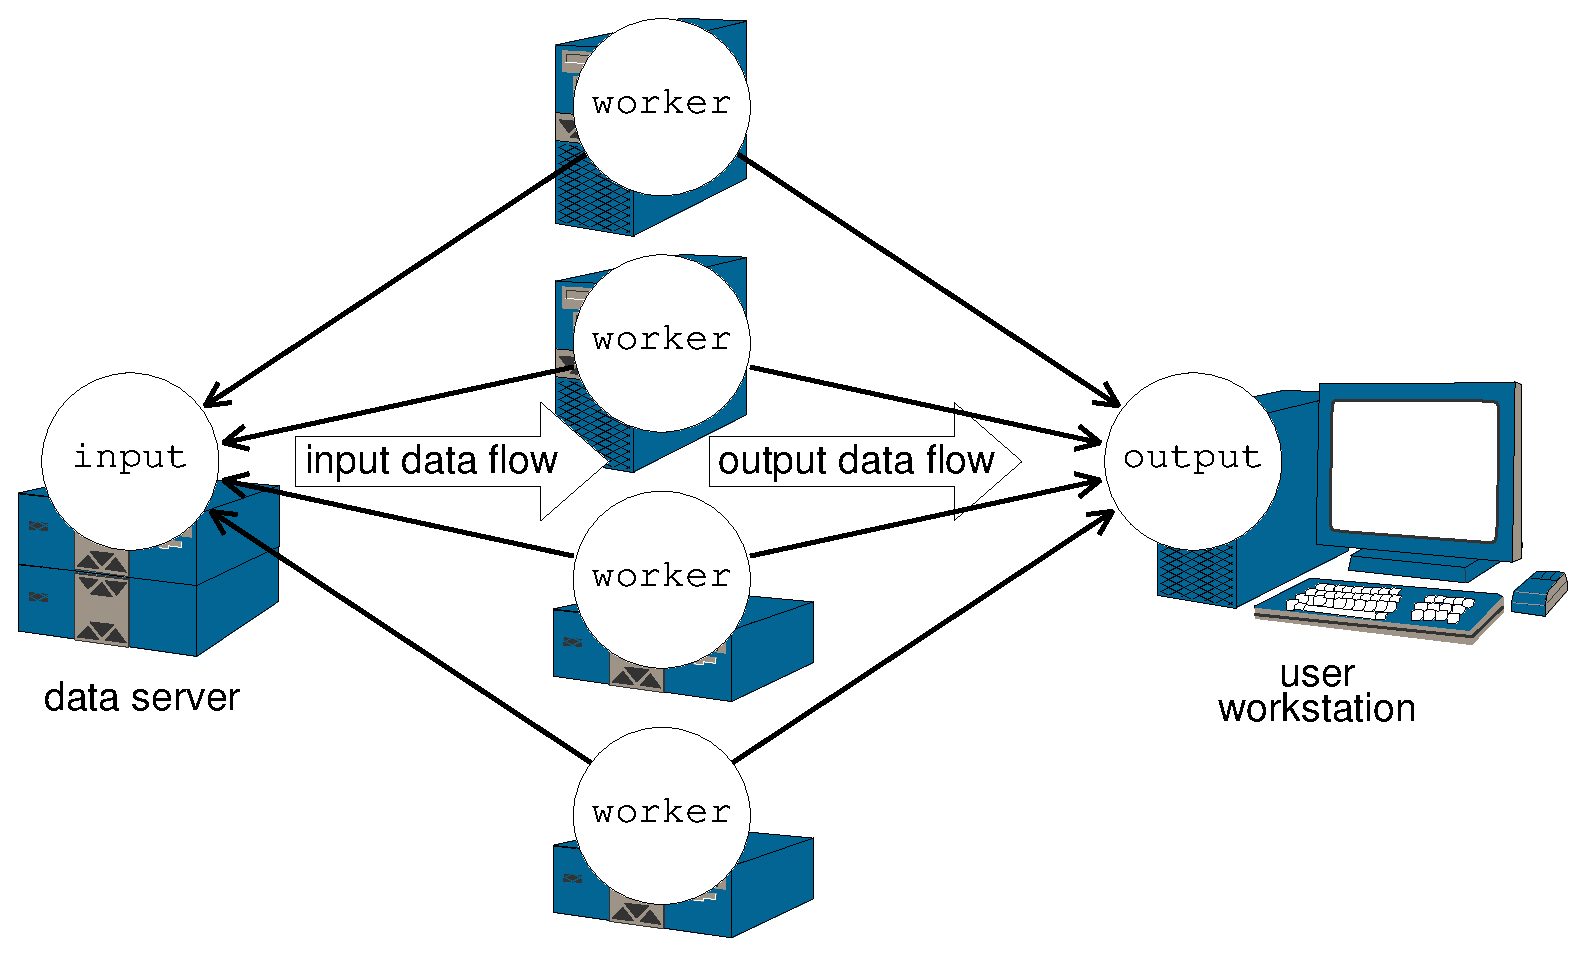
\includegraphics[scale=0.5]{fig_use_scenario.eps}
	\label{fig_use_scenario}
\end{figure}


To share the reference of a parallel object, POP-Java allows parallel objects
to be arbitrarily passed from one place to another as arguments of method
invocations.

\pagebreak
\subsection{Invocations semantics}
\label{semantic}
Syntactically, method invocations on parallel objects are identical to those
on traditional sequential objects. However, to each method of a parallel
object, one can associate different invocation semantics. Invocation
semantics are specified by programmers when declaring methods of
parallel objects. These semantics define different behaviors for the
execution of the method as described below (example of syntax in chapter \ref{dev})

\begin{itemize}

\item \emphasis{Interface semantics}, the semantics that affect the caller
of the method:
	\subitem \textbf{Synchronous invocation}: the caller waits until the
	execution of the called method on the remote object is terminated.
  This corresponds to the traditional method invocation.

	\subitem \textbf{Asynchronous invocation}: the invocation returns
	immediately after sending the request to the remote object.
	Asynchronous invocation is important to exploit the parallelism.
	However, as the caller does not wait the end of the execution of the
	called method, no computing result is available. This excludes
	asynchronous invocations from producing results. Results can be
	actively returned to the caller object using a callback to the caller.
	To do so the called object must have a reference to the caller object.
	This reference can be passed as an argument to the called method
	(see figure[\ref{fig_inv_async}]).




\begin{figure}[ht]
	\caption{Callback method returning values from an asynchronous call}
  	\centering
	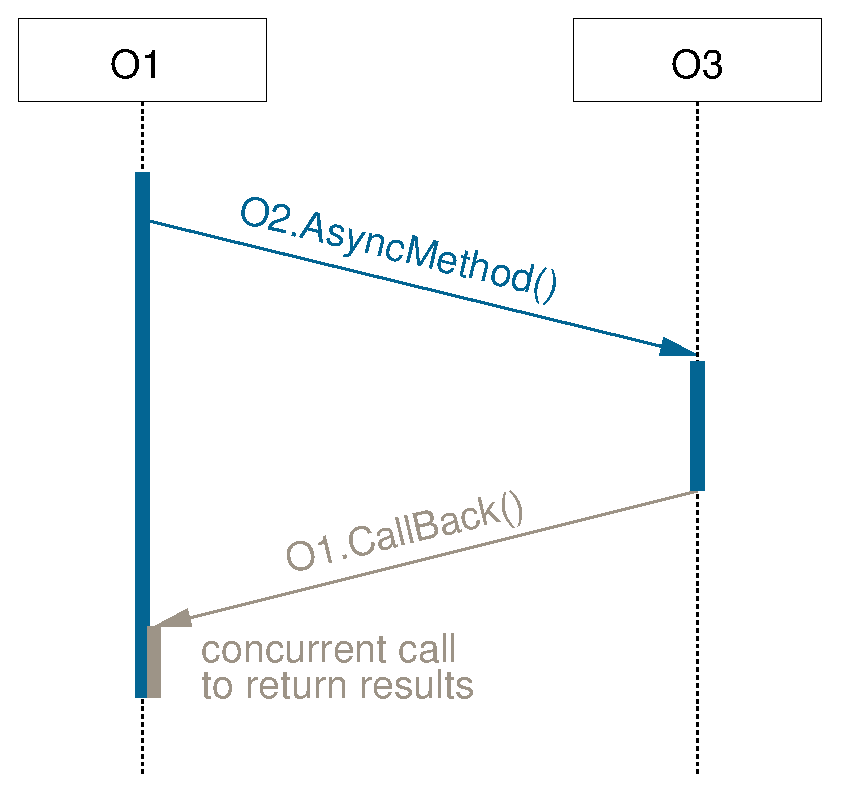
\includegraphics[scale=0.5]{fig_inv_async.eps}
	\label{fig_inv_async}
\end{figure}



\item \emphasis{Object-side semantics}, the semantics that affect the order
 of the execution of methods in the called parallel object:

	\subitem \textbf{A mutex call} is executed after completion of all calls previously arrived.
	
	\subitem \textbf{A sequential call} is executed after completion of all sequential and
	mutex calls previously arrived.

	\subitem \textbf{A concurrent call} can be executed concurrently (time sharing) with other
	concurrent or sequential calls, except if mutex calls are pending or executing.
	In the later case he is executed after completion of all mutex calls previously
	arrived.

\end{itemize}

In a nutshell, different object-side invocation semantics can be
expressed in terms of atomicity and execution order. The mutex
invocation semantics guarantees the global order and the atomicity of
all method calls. The sequential invocation semantics guarantees only
the execution order of sequential methods. Concurrent invocation
semantics guarantees neither the order nor the atomicity.


\begin{figure}[ht]
	\caption{Example of different invocation requests}
  	\centering
	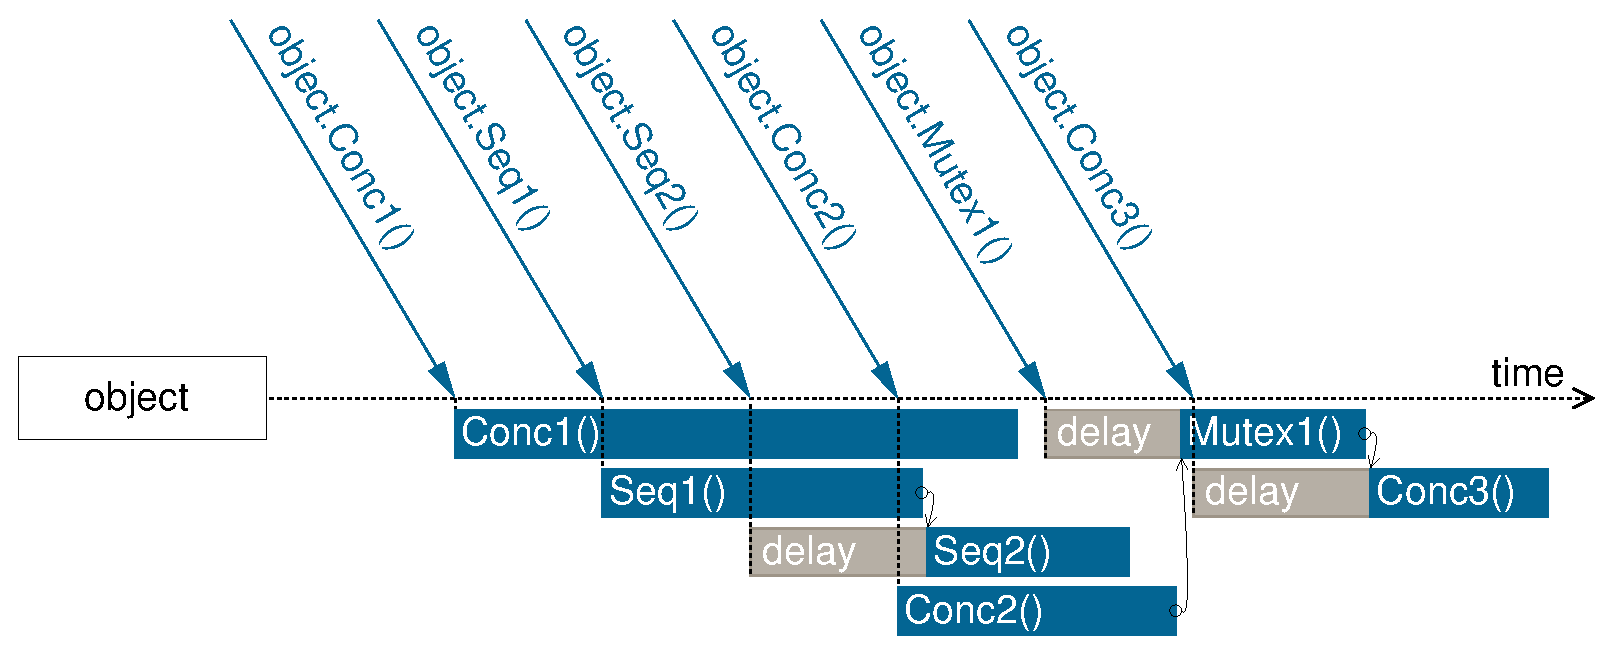
\includegraphics[scale=0.5]{fig_inv_semantics.eps}
	\label{fig_inv_semantics}
\end{figure}


Figure[\ref{fig_inv_semantics}] illustrates different method invocation
semantics. Sequential invocation \texttt{Seq1()} is served immediately,
running concurrently with \texttt{Conc1()}. Although the sequential
invocation \texttt{Seq2()} arrives before the concurrent invocation
\texttt{Conc2()}, it is delayed due to the current execution of
\texttt{Seq1()} (no order between concurrent and sequential invocations).
When the mutex invocation \texttt{Mutex1()} arrives, it has to wait for
other running methods to finish. During this waiting, it also blocks
other invocation requests arriving afterward (\texttt{Conc3()}) until
the mutex invocation request completes its execution (atomicity and
barrier).


\subsection{Parallel Object Allocation}
\label{allocation}
The first step to allocate a new object is the selection of an adequate
placeholder. The second step is the object creation itself. Similarly,
when an object is no longer in use, it must be destroyed in order to
release the resources it is occupying in its placeholder. The POP-C++
runtime system provides automatic placeholder selection, object
allocation, and object destruction. This automatic features result in a
dynamic usage of computational resources and gives to the applications
the ability to adapt to the changes in both the environment and the user
behavior.\s

The creation of POP-Java parallel objects is driven by high-level
requirements on the resources where the object should lie (see section
\ref{requirement}). If the programmer specifies these requirements
they are taken into consideration by the runtime system for the transparent 
object allocation. The allocation process consists of three phases: first, the system finds a suitable resource, where the
object will lie; then the object code is transmitted and executed on
that resource; and finally, the corresponding interface is created and
connected to the object.


\subsection{Requirement-driven parallel objects}
\label{requirement}
Parallel processing is increasingly being done using distributed
systems, with a strong tendency towards web and global computing.
Efficiently extract high performance from highly heterogeneous and
dynamic distributed environments is a challenge today. POP-C++ and POP-Java were
conceived under the belief that for such environments, high performance
can only be obtained if the two following conditions are satisfied:

\begin{itemize}

\item The application should be able to adapt to the environment;

\item The programming environment should somehow enables objects
to describe their resource requirements.

\end{itemize}

The application adaptation to the environment can be fulfilled by
multilevel parallelism, dynamic utilization of resources or adaptive
task size partitioning. One solution is to dynamically create parallel
objects on demand.

Resource requirements can be expressed by the quality of service that
objects require from the environment. Most of the systems offering
quality of service focus on low-level aspects, such as network bandwidth
reservation or real-time scheduling. Both POP-C++ and POP-Java integrate the programmer
requirements into parallel objects in the form of high-level resource
descriptions. Each parallel object is associated with an object
description that depicts the characteristics of the resources needed to
execute the object. The resource requirements in object descriptions are
expressed in terms of:

\begin{itemize}

\item Resource (host) name (low level description, mainly used to
develop system services).

\item The maximum computing power that the object needs (expressed in
MFlops).

\item The maximum amount of memory that the parallel object consumes.

\item The expected communication bandwidth and latency.

\item The preferred communication protocol.

\item The preferred encoding protocol.


\end{itemize}

An object description can contain several items. Each item corresponds
to a type of characteristics of the desired resource. The item is
classified into two types: strict item and non-strict item. A strict
item means that the designated requirement must be fully satisfied. If
no satisfying resource is available, the allocation of parallel object
fails. Non-strict items, on the other hand, give the system more freedom
in selecting a resource. Resource that partially match the requirements
are acceptable although a full qualification resource is  preferable.
For example, a certain object has a preferred performance 150MFlops
although 100MFlops is acceptable (non-strict item), but it need memory
storage of at least 128MB (strict item).\s

The construction of object descriptions occurs during the parallel
object creation. The programmer can provide an object description to
each object constructor. The object descriptions can be parametrized by
the arguments of the constructor. Object descriptions are used by the
runtime system to select an appropriate resource for the object. Some example 
of the syntax of object descriptions can be found in the section \ref{dev:objdesc}.\s

It can occur that, due to some changes on the object data or some
increase of the computation demand, an object description needs to be
re-adjusted during the life time of the parallel object. If the new
requirement exceeds some threshold, the adjustment could cause the
object migration. The current implementations of POP-C++ and POP-Java do not support
object migration yet.


% POP-JAVA Dev
%\emptypage
\pagebreak
\section{Developing POP-Java application}
\label{dev}

The POP model (chapter \ref{popmodel}) is a suitable programming model for large heterogeneous distributed environments but it should also remain as close as possible to traditional object oriented programming. Parallel objects of the POP model generalize sequential objects, keep the properties of object oriented programming (data encapsulation, inheritance and polymorphism) and add new properties.\s

The POP-Java language is an extension of Java that implements the POP model. Its syntax remains as close as possible to standard Java so that Java programmer can easily learn it and existing Java libraries can be parallelized without much effort. Changing a sequential Java application into a distributed parallel application is rather straightforward. POP-Java is also very close to POP-C++ so that POP programmer can use both system easily.\s

Parallel objects are created using parallel classes. Any object that instantiates a parallel class is a parallel object and can be executed remotely. To help the POP-C++ runtime to choose a remote machine to execute the remote object, programmers can add object description information to each constructor of the parallel object. In order to create parallel execution, POP-Java offers new semantics for method invocations. These new semantics are indicated thanks to new POP-Java keywords. This chapter describes the syntax of the POP-Java programming language and presents the main tools available in the POP-Java system.


\subsection{Parallel objects}
POP-Java parallel objects are a generalization of sequential objects. Unless the term sequential object is explicitly specified, a parallel object is simply referred as an object in the rest of this chapter.

\subsubsection{Create a parallel class}
Developing POP-Java application mainly consists of designing an implementing parallel classes.
The declaration of a parallel class is the same as a standard Java class declaration, but it has to be annotated
with the annotation \textbf{@POPClass}.
The parallel class can extend another parallel class but not a sequential class.\s

\textbf{Simple parallel class declaration}
\begin{lstlisting}
@POPClass
public class MyParallelClass {
	//Implementation
}
\end{lstlisting}\s

\textbf{Parallel class declaration with an inheritance}
\begin{lstlisting}
@POPClass
public class MyParallelClass extends AnotherParallelClass {
	//Implementation
}
\end{lstlisting}\s

As Java allows only the single inheritance, a parallel class can only inherit from \textbf{one} other parallel class.
The Java language also impose that the file including the parallel class has the same name than the parallel class.\s

POP-Java imposes also one restrictions. The parallel class must be declared and implemented in a file with \textbf{.pjava} extension.
For example, the parallel class \textit{MyParallelClass} declared before, must be in a file \textbf{MyParallelClass.pjava}.\s

Parallel classes are very similar to standard Java classes. As POP-Java has some different behavior, some restrictions applied to the parallel classes : 
\begin{itemize}
\item All attributes in a parallel class must be protected or private
\item The objects do not access any global variable
\item A parallel class does not contain any static attributes or static methods
\end{itemize}


\subsubsection{Creation and destruction}
The object creation process consists of several steps: locating a resource satisfying the object description (resource discovery), transmitting and executing the object code, establishing the communication, transmitting the constructor arguments and finally invoking the corresponding object constructor. Failures on the object creation will raise an exception to the caller. Section \ref{exception} will describe the POP-Java exception mechanism.\s

As a parallel object can be accessible concurrently from multiple distributed locations (shared object), destroying a parallel object should be carried out only if there is no other reference to the object. POP-Java manages parallel objects' life time by an internal reference counter. A counter value of 0 will cause the object to be physically destroyed. \s

Syntactically, the creation of a parallel object is identical to the one in Java. A parallel object can be created by using the standard new operator of Java.


\subsubsection{Parallel class methods}
Like sequential classes, parallel classes contain methods and attributes.
Method can be public or private but attribute must be either protected or private.
For each public method, the programmer must define the invocation semantics.
These semantics, described in section \ref{semantic}, are specified by an annotations.

\begin{itemize}
\item \textbf{Interface side} : These semantics affect the caller side.
\subitem sync : Synchronous invocation. 
\subitem async : Asynchronous invocation.
\item \textbf{Object side} : These semantics affect the order of the class inside the object itself.
\subitem seq : Sequential invocation
\subitem conc : Concurrent invocation
\subitem mutex : Mutual exclusive invocation
\end{itemize}

The combination of the interface and object-side semantics defines the overall semantics of a method. There
are 6 possible combinations of the interface and object-side semantics, resulting in 6 annotions:

\begin{lstlisting}
@POPSyncConc
@POPSyncSeq
@POPSyncMutex
@POPAsyncConc
@POPAsyncSeq
@POPAsyncMutex
\end{lstlisting}
\pagebreak
For example, a synchronous concurrent method returning an int value must be declared as follow : 
\begin{lstlisting}
@POPSyncConc
public int myMethod(){
	return myIntValue;
}
\end{lstlisting}

A method declared as asynchronous must have its return type set to void. Otherwise, the compiler will raise an error.


\subsubsection{Object description}
\label{dev:objdesc}
Object descriptions are used to describe the resource requirements for the execution of an object.
Object descriptions are declared along with parallel object constructor declarations.
The object description can be declared in a static way as an annotation of the constructor, or in a dynamic way
as an annotation on the parameters of the constructor. First an example of a static annotation:

\begin{lstlisting}
@POPObjectDescription(url="localhost")
public MyObject(){
}
\end{lstlisting}\s

and now a dynamic example:
\begin{lstlisting}
public MyObject(@POPConfig(Type.URL) String host){
}
\end{lstlisting}\s

Currently only the url annotation is implemented, allowing to specify the url/IP of the machine on which the POP-Object is executed.
If the annotation is not set, POP-Java will use the POP-C++ jobmanager to find a suitable machine.

\begin{comment}
Here are the list of accepted resource requirements expressions in the current POP-Java version : 

\begin{itemize}
\item od.power(exact, lbound) : Specify the computing power needed (in Mflops).
\item od.memory(exact, lbound) : Specify the memory size needed (in MB).
\item od.bandwidth(exact, lbound) : Specifiy the bandwidth (in Mb/s) needed for the connection.
\item od.encoding(string) : Specify the encoding ("raw" or "xdr") used for the data transfer.
\item od.protocol(string) : Specify the protocol (only "socket" for the moment) used for the network connection.
\end{itemize}

Both \textit{exact} and \textit{lbound} terms are numeric expressions and \textit{string} is a standard Java string expression.
The object descriptions allowing two values (\textit{exact} and \textit{lbound}) have a priority set to the first value.
If no resource are found for this specified \textit{exact} value, the \textit{lbound} value will be used.\s

An example of object description is given in the following code.
The constructor for the parallel object \textit{MyParallelClass} requires the computing power of "p" Mflops or at least 80 Mflops.
The memory requirement is set to 100MB or at least 60MB.


\begin{lstlisting}
public parclass MyParallelClass {
	public MyParallelClass(float p) @{ od.power(p, 80); 
	  od.memory(100,60); }{
		
	}
}
\end{lstlisting}\s



The object description are used by the POP-C++ runtime system to find suitable resource for executing the parallel object.
Matching between object descriptions and resources is carried out by a multi-layer filtering technique: first, each expression (item) in every object descriptor will be evaluated and categorized (e.g., power, memory, network).
Then, the matching process consists of several layers: each layer filters single category within the object descriptors and performs matching on that category. Finally, if an object descriptor pass all filters, the object is assigned to that resource.\s

If no suitable resource is found to execute the object then an exception is raised.
\end{comment}

\subsubsection{Data marshaling and IPOPBase}
When calling a remote methods, the arguments must be transferred to the object being called (the same happens for the return value and the exception).  In order to operate with different memory spaces and different architecture, data is marshaled into a standard format prior to be send to remote objects. All data passed is serialized (marshaled) at the caller side an deserialized (unmarshaled) at the called side. \s

With POP-Java all primitive types, primitive types arrays and parallel classes can be passed without any trouble to another parallel object. This mechanism is transparent for the programmer.\s

If the programmer want to pass a special object to or between parallel classes, this object must implement the IPOPBase interface from the POP-Java library. This library is located in the installation directory (\textit{POPJAVA\_LOCATION/JarFile/popjava.jar}). By implementing this interface, the programmer will have to override the two following methods : 

\begin{lstlisting}
@Override
public boolean deserialize(Buffer buffer) {
  return true;
}

@Override
public boolean serialize(Buffer buffer) {
  return true;
}
\end{lstlisting}\s

These methods will be called by the POP-Java system when an argument of this type need to be serialized or deserialized. As the object will be reconstruct on the other side and after the values will be set to it by the deserialize method, any class implementing the IPOPBase interface must have a default constructor.\s

\pagebreak
The code below shows a full example of a class implementing the IPOPBase interface.


\begin{lstlisting}
import popjava.buffer.Buffer;
import popjava.dataswaper.IPOPBase;

public class MyComplexType implements IPOPBase {
	private int theInt;
	private double theDouble;
	private int[] someInt;
	
	public MyComplexType(){}
	
	public MyComplexType(int i, double d, int[] ia){
		theInt = i;
		theDouble = d;
		someInt = ia;
	}
	
	@Override
	public boolean deserialize(Buffer buffer) {
		theInt = buffer.getInt();
		theDouble = buffer.getDouble();
		int size = buffer.getInt();
		someInt = buffer.getIntArray(size);
		return true;
	}

	@Override
	public boolean serialize(Buffer buffer) {
		buffer.putInt(is);
		buffer.putDouble(ds);
		buffer.putIntArray(ias);		
		return true;
	}
}
\end{lstlisting}

\subsection{POP-Java behavior}
This section aims to explain to difference between the standard Java behavior and the POP-Java behavior.\s

As in standard Java, the primitive types will not be affected by any manipulations inside a methods. The objects will be affected only if the method semantic is “Synchronous”. In fact, POP-Java serialize the method arguments to pass them on the object-side. Once the method work is done, the arguments are serialize once again to be send back to the interface-side. If the method semantic is “Synchronous”, the interface-side will deserialize
the arguments and replace the local ones by the deserialized arguments. If the method semantic is
“Asynchronous”, the interface-side will not wait for any answer from the object-side. It's important to understand this small difference when developing POP-Java application.

\subsection{Exception handling}
\label{exception}
Errors can be efficiently handled using exceptions. Instead of handling each error separately based on an error code returned by a function call, exceptions allow the programmer to filter and centrally manage errors trough several calling stacks. When an error is detected inside a certain method call, the program can throw an exception that will be caught somewhere else.\s

The implementation of exception in non-distributed applications, where all components run within the same memory address space is fairly simple. The compiler just need to pass a pointer to the exception from the place where it is thrown to the place where it is caught.  However, in distributed environments where each component is executed in a separated memory address space (and eventually data are represented differently due to heterogeneity), the propagation of exception back to a remote component is complex.

\begin{figure}[ht]
\caption{Exception handling example}
\center
\label{fig:exception}
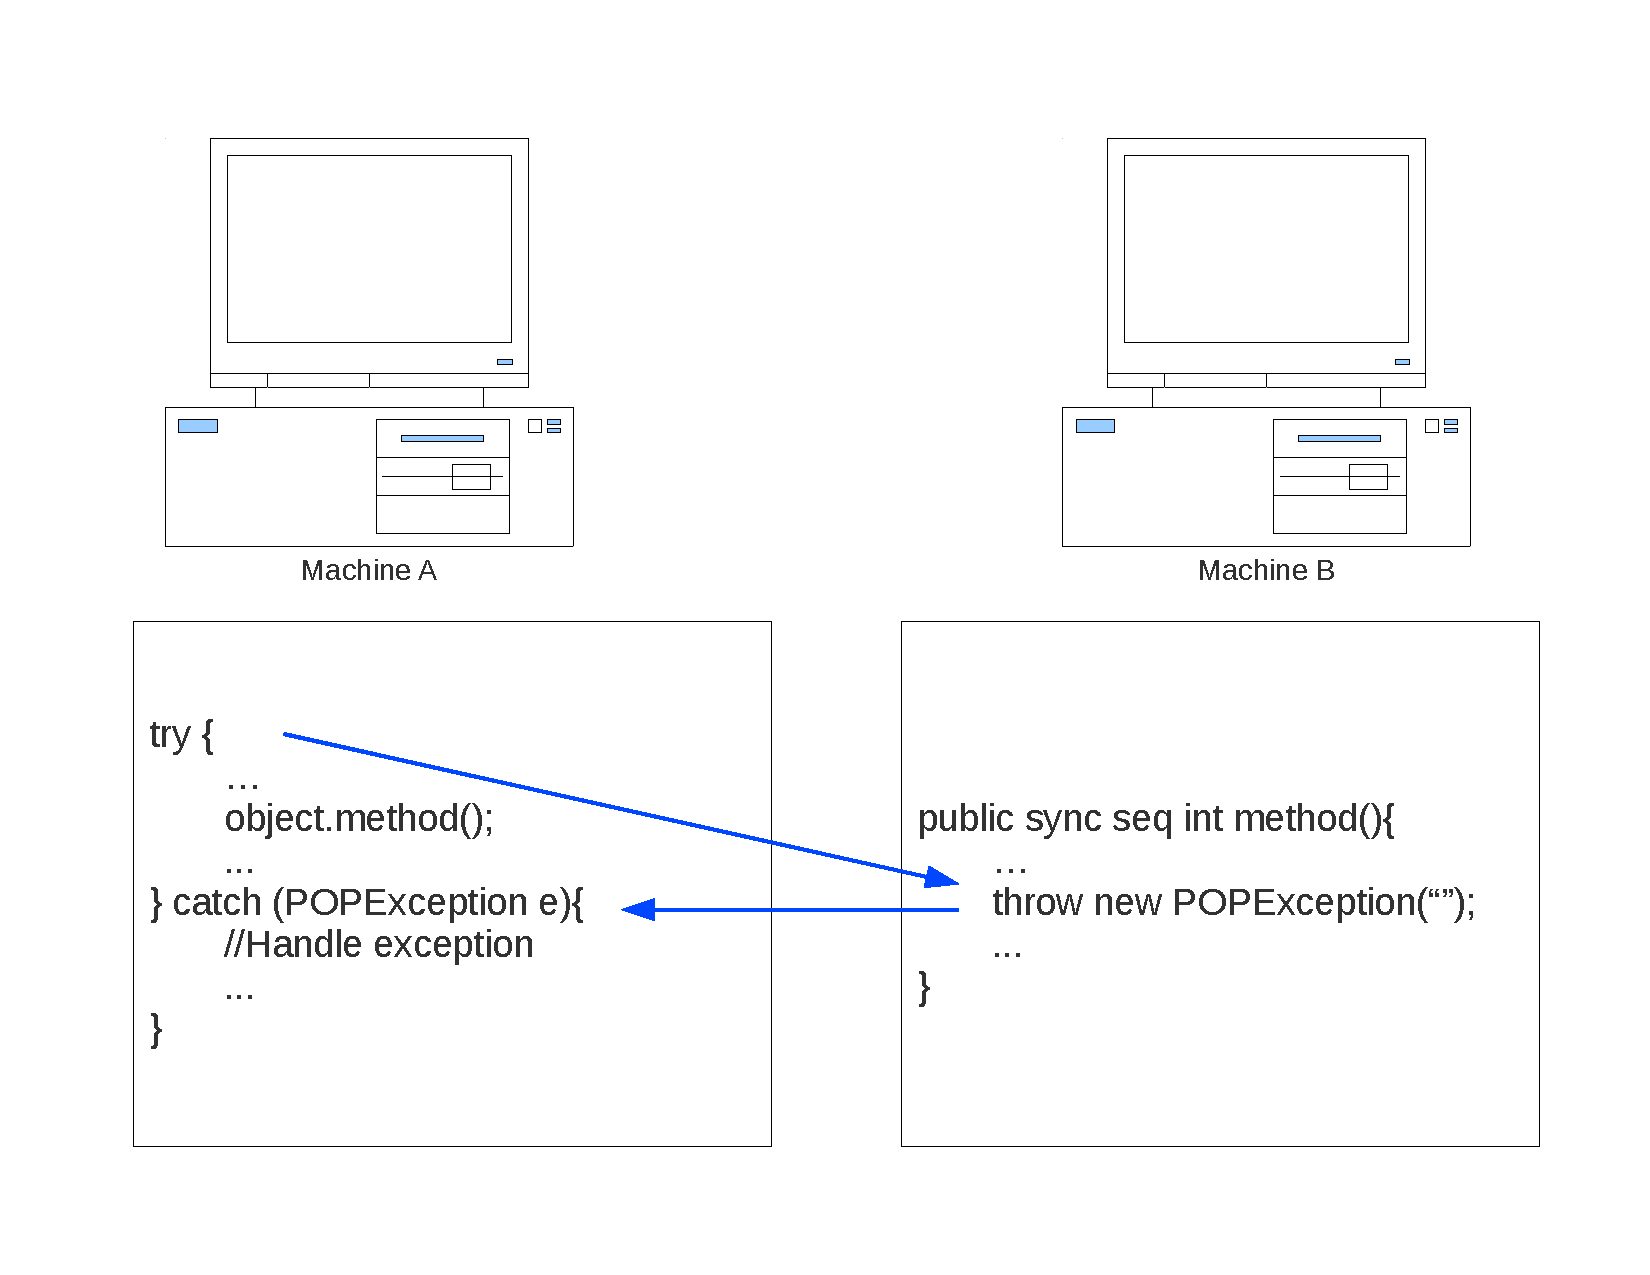
\includegraphics[scale=0.3]{exception.pdf}
\end{figure}

POP-Java supports transparent exception propagation. Exceptions thrown in a parallel object will be automatically propagated back to the remote caller (figure[\ref{fig:exception}]). The current POP-Java version allows the following types of exceptions : 
\begin{itemize}
\item Exception
\item POPException
\end{itemize}

The invocation semantics of POP-Java affect the propagation of exceptions. For the moment, only synchronous methods can propagate the exception. Asynchronous methods will not propagate any exception to the caller. POP-Java current behavior is to abort the application execution when such exception occurs. 




% COMPILE AND RUN
\pagebreak
\section{Compile and run a POP-Java application}
\label{compileandrun}
This chapter explain the POP-Java compilation process, the POP-Java application launching process and the tools related to those processes. The structure of this chapter is as follows : The first section explains the compilation process and the special compiler for POP-Java. The second describes the application launching tools. The third one aims to help the programmer to understand the importance of the object map and the object map generator in the POP-Java application launching process. Finally, a full example is explained to pass trough the whole process. 


\subsection{The POP-Java compiler}
POP-Java has its own compilation process. As POP-Java applications are written in the POP-Java language, the programmer have to use the POP-Java compiler to compile its application. The figure [\ref{fig:popjava_compiler}] shows the POP-Java compilation process. The POP-Java source files will be converted in standard Java source files by a specific parser and code generator. These Java source files will be compiled with the POP-Java library and produce compiled class files or a Java archive file (JAR). \s


\begin{figure}[ht]
	\caption{POP-Java compilation process}
  	\centering
	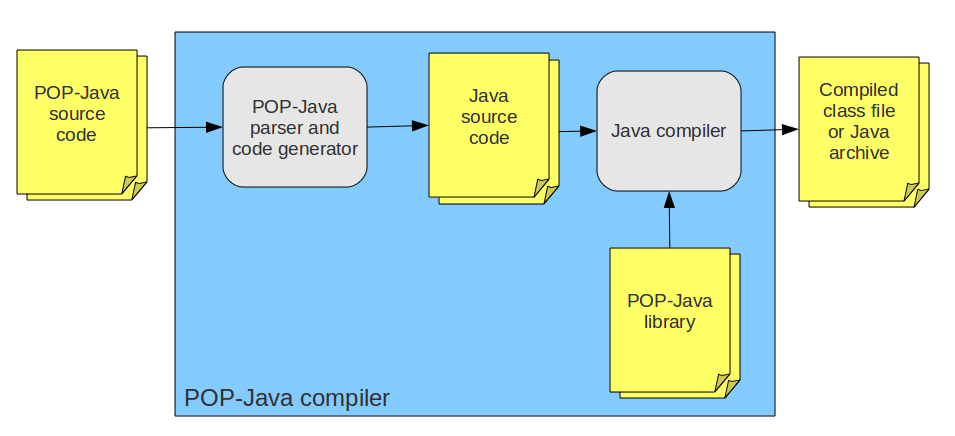
\includegraphics[scale=0.6]{popjcompiler.png}
	\label{fig:popjava_compiler}
\end{figure}

The POP-Java compiler will parse and generate new source file only for the files with .pjava extension. Due to that, it is very important the main class and the parallel classes have this extension and not the standard .java extension.\s

The POP-Java compiler is accessible trough the command "popjc". The command syntax is as follow : 
\begin{lstlisting}
popjc <options> <files>
\end{lstlisting}\s

Options
\begin{itemize}
\item -n or --noclean : Do not clean the temporary files generated by the parser and code generator. 
\item -p or --popcpp : Use the specified additional informations XML file for the compilation (See chapter \ref{mixed}).
\item -j or --jar : Compile the source files in a JAR file. Name of the JAR must be specified.
\item -v or --verbose : Print additional information during the compilation process. 
\item -c or --classpath : Add class file or JAR file to the compilation
\item -x or --xmlpopcpp : Generate the XML additional information file with the specified source files (See chapter \ref{mixed}).
\item -g or --generate : Generate the POP-C++ partial implementation from the specified source file (See chapter \ref{mixed}). Not implemented in the current version.
\end{itemize}

The files in the command line are the ones to compile (.pjava or .java). The command help is available in the appendix \ref{popjc_help}.


\subsection{The POP-Java application launcher}
To help POP-Java programmer, POP-Java provide an application launcher that simplify the launch of a POP-Java application. This application launcher is named "popjrun" and is used with the following syntax : 

\begin{lstlisting}
popjrun <options> [<objectmap>] <MainClass> <arguments>
\end{lstlisting}\s

Here is an explanation of the arguments to provide to the POP-Java application launcher : 

\begin{itemize}
\item \textbf{options} : in the current version there is only one option "-c" or "--classpath" that allow the programmer to add some class path for the execution of the POP-Java application. The different class paths must be separated with a semicolon.
\item \textbf{objectmap} : this informations is not mandatory. If it's provided, the object map inform the runtime system about the location of the different compiled parallel classes of the application. If it's not provided, the default object map (located under : \textit{POPJAVA\_LOCATION}/etc/defaultobjectmap.xml) will be used. More information give in the section \ref{objectmap}.
\item \textbf{MainClass} : this is a main class of the POP-Java application.
\item \textbf{arguments} : there are the arguments of the program
\end{itemize}


\subsection{The POP-Java object map and object map generator}
\label{objectmap}
The object map is an XML file that informs the POP-C++ runtime about the location of the different compiled parallel classes of the application. This file can be given to the "popjrun" tool. If the programmer do not give this file, the default object map located in \textit{POPJAVA\_LOCATION}/etc/ will be used. \s

The object map can be generated with the POP-Java application launcher. By using the option "-l" or "--listlong" and giving the class files or the JAR file, the object map will be printed to the standard output. The easiest way to save this file is to redirect the output into the desired file.\s

Here are the command used for our example : \s

\textbf{Compiled classes}
\begin{lstlisting}
popjrun --listlong Parclass1.class:Parclass2.class > objectmap.xml
\end{lstlisting}\s

\textbf{JAR file}
\begin{lstlisting}
popjrun --listlong parclasses.jar > objectmap.xml
\end{lstlisting}

\pagebreak
\subsection{Full example}
This section shows how to write, compile and launch a POP-Java application by using a simple example. The POP-Java application used in this example includes only one parallel class. All sources of this example can be found in the directory "examples/integer" from the POP-Java distribution.

\subsubsection{Programming}
When we start to develop a POP-Java application the main part is the parallel classes. The figure [\ref{fig:code_integer.pjava}] shows the parallel class implementation. As we can see this class use special POP-Java keywords. In the line 1, the parclass keyword specifies that this class is a parallel class. The constructor declaration includes an object description (line 4). The method declarations includes the invocation semantics (line 8, 12 and 16). The method "add" (line 16) receive another parallel object as a parameter and it's transparent for the programmer.

\begin{figure}[ht]
\caption{File Integer.pjava}
\label{fig:code_integer.pjava}
\begin{lstlisting}
1:  @POPClass
2:  public class Integer {
3:    private int value;
4:	
5:        @POPObjectDescription(url="localhost")
6:	  public Integer(){
7:	    value = 0;	
8: 	  }
9: 	
10:	  @POPSyncConc
11:	  public int get(){
12:	    return value	
13:	  }
14:	
15:	  @POPAsyncSeq
16:	  public void set(int val){
17:	    value = val;	
18:	  }
19:	
20:       @POPAsyncMutex
21:	  public void add(Integer i){
22:	    value += i.get();	
23:	  }
24:	}
\end{lstlisting}
\end{figure}

\pagebreak
Once the parallel class is implemented, we can write a main class that use this parallel class.
The figure [\ref{fig:code_testinteger.pjava}] shows the code of the main class. The code of the main class is pure Java code.
However, this code must be declared in a file with ".pjava" extension to be considered by the POP-Java compiler.
The instantiation (lines 3-4) and the method calls (lines 5-9) are transparent for the programmer.

\begin{figure}[ht]
\caption{File TestInteger.pjava}
\label{fig:code_testinteger.pjava}
\begin{lstlisting}
1: 	public TestInteger {
2: 	  public static void main(String[] args){
3:	    Integer i1 = new Integer();
4:	    Integer i2 = new Integer();
5:	    i1.set(23);
6:	    i2.set(25);
7:	    System.out.println("i1=" + i1.get());
8:	    System.out.println("i2=" + i2.get());
9:	    i1.add(i2);
10:	    int sum =  i1.get();
11:	    System.out.println("i1+i2 = "+sum);
12:	    if(sum==48)
13:	      System.out.println("Test Integer Successful");
14:	    else
15:	      System.out.println("Test Integer failed");
16:	    }
17:	}
\end{lstlisting}
\end{figure}


\subsubsection{Compiling}
The POP-Java compiler can generate two kind of compiled code. The first is the standard Java compiled class file (.class). The second is the Java archive (JAR) file. Here are the two commands to compile the example application.\s

\textbf{Compiling as .class files}
\begin{lstlisting}
popjc Integer.pjava TestInteger.pjava
\end{lstlisting}\s

\textbf{Compiling as a JAR file}
\begin{lstlisting}
popjc -j myjar.jar Integer.pjava TestInteger.pjava
\end{lstlisting}

\subsubsection{Create the object map}
Before running the example application, the programmer needs to generate the object map. The object map will be given to the POP-Java launcher. This file will inform the POP-C++ runtime system where to find the compiled files. The POP-Java launcher has a specific option to generate this file from the compiled files (.class) or the JAR file (.jar). Here is the command used for our example :

\begin{lstlisting}
popjrun --listlong Integer.class > objmap.xml
\end{lstlisting}\s

The command will generate the XML file and print it on the standard output. To save this file, we redirect the output in a file named objmap.xml. This file contains the following XML code (the path specified in the element CodeFile will be different on your computer) : 

\begin{lstlisting}
<CodeInfoList>
  <CodeInfo>
    <ObjectName>Integer</ObjectName>
    <CodeFile Type="popjava">
      /home/clementval/pop/popjava-1.0/example/integer/</CodeFile>
    <PlatForm>*-*</PlatForm>
  </CodeInfo>
</CodeInfoList>
\end{lstlisting}


\subsubsection{Running}
Once the POP-Java application is compiled and the object map is generated, the application can be run. A POP-Java application is a pure Java application at the end and could be run with the standard java program. In order to make this running easier for the programmer, POP-Java include an application launcher. Here are the command to use to run the POP-Java application example : \s

\textbf{POP-Java application compiled as .class files}
\begin{lstlisting}
popjrun objectmap.xml TestInteger
\end{lstlisting}\s

\textbf{POP-Java application compiled as .jar file}
\begin{lstlisting}
popjrun -c myjar.jar objectmap.xml TestInteger
\end{lstlisting}\s

\textbf{Application output}\\
Here is what we should have as the application output : 
\begin{lstlisting}
i1=23
i2=25
i1+i2=48
Test Integer Successful 
\end{lstlisting}\s

If we have any problems with the compilation or the launching of the application, please see the chapter \ref{trouble}.


% POP-Java POP-C++
%\emptypage
\pagebreak
\section{Developing POP-Java and POP-C++ mixed application}
\label{mixed}
%%%%%%%%%%%%%%%%%%%%%%%%%%%%%%%%%%%%%%%%%%%%%%%%%%%%%%%%%%%%%%%%%
% POP-JAVA AND POP-C++
%%%%%%%%%%%%%%%%%%%%%%%%%%%%%%%%%%%%%%%%%%%%%%%%%%%%%%%%%%%%%%%%%
\subsection{POP-Java and POP-C++ interoperability}
POP-Java can use POP-C++ parallel classes and POP-C++ can also use POP-Java parallel classes. This chapter will explain everything the programmer needs to know to develop mixed POP application. 


\subsection{Restrictions}
As Java and C++ are different languages, there are some restrictions. In this section, all the restrictions or programming tips will be given.

\subsubsection{Java primitives}
As Java primitives are always passed by value, the is no way to modify a Java primitive in a POP-C++ object. In pure POP-C++ the programmer can deal with the passing by reference but not in POP-Java.

\subsubsection{Parameters passing}
Some parameters cannot be passed from a POP-Java application to a POP-C++ parallel object and vice versa. The list below explain the restrictions on certain primitive types. The Java primitive types are taken as the basis.

\begin{itemize}
\item \textbf{byte} : This type does not exist in C++ so it's not possible to pass a byte.
\item \textbf{long} : The Java long is coded on 8 bytes as it's coded on 4 bytes with C++. Some unexpected behavior can occurred.
\item \textbf{char[]} : The char array cannot be used in the current version of POP-Java with POP-C++ parallel classes.
\end{itemize}

\subsubsection{Dealing with array}
Passing arrays from POP-Java to POP-C++ is a bit tricky. As POP-Java and POP-C++ do not behave the same with array, the programmer must be aware of the way to pass the array. Here is a example of a method with an array as parameter.\s

\textbf{The method declaration in POP-C++}\\
In POP-C++, the programmer must give the array size to the compiler.
\begin{lstlisting}
sync seq void changeIntArray(int n, [in, out, size=n] int *i);
\end{lstlisting}\s

\textbf{Method declaration in POP-Java}\\
As POP-C++ will need the size of the array, POP-Java must declare this size as well.
\begin{lstlisting}
@POPSyncSeq
public void changeIntArray(int n, int[] i){}
\end{lstlisting}\s

\textbf{Method call from POP-Java}\\
In the POP-Java application, the programmer need to give the array size in the method call.
\begin{lstlisting}
p.changeIntArray(iarray.length, iarray);
\end{lstlisting}



%%%%%%%%%%%%%%%%%%%%%%%%%%%%%%%%%%%%%%%%%%%%%%%%%%%%%%%%%%%%%%%%%
% POP-JAVA APPLICATION WITH POP-C++ PARCLASS
%%%%%%%%%%%%%%%%%%%%%%%%%%%%%%%%%%%%%%%%%%%%%%%%%%%%%%%%%%%%%%%%%
\pagebreak
\subsection{POP-Java application using POP-C++ parallel objects}
This section will teach the programmer how to develop a POP-Java application with a POP-C++ parallel class. The same example of the parallel class Integer will be used.  For more details about the POP-C++ programming please have a look to "Parallel Object Programming C++ - User and Installation Manual"\cite{popc_intro}. In the following example, the main class used is the same as the one shown in the figure[\ref{fig:code_testinteger.pjava}]. All the sources can be found in the directory "example/mixed1" of the POP-Java distribution.

\subsubsection{Develop the POP-C++ parallel class}
First, the programmer needs to write the parallel class in POP-C++ as it should be for a POP-C++ application. The figure[\ref{fig:file_integer.ph}] shows the header file of the parclass Integer. There is two rules to follow when the programmer develop a POP-C++ parallel class for POP-Java usage.
\begin{enumerate}
\item The parclass must declare a classuid.
\item The methods must be declared in alphabetics order.
\end{enumerate}

\begin{figure}[ht]
	\caption{File integer.ph}
	\label{fig:file_integer.ph}
\begin{lstlisting}
parclass Integer
{
  classuid(1000);
public:	
  Integer();
  ~Integer();

  mutex void Add(Integer &other);
  conc int Get();
  seq async void Set(int val);

private:
  int data;
};
\end{lstlisting}
\end{figure}

\pagebreak
The figure[\ref{fig:file_integer.cc}] shows the implementation of the parallel class Integer. There is no important information in this file for the POP-Java usage.

\begin{figure}[ht]
	\caption{File integer.cc}
	\label{fig:file_integer.cc}
\begin{lstlisting}
#include <stdio.h>
#include "integer.ph"
#include <unistd.h>

Integer::Integer() {
  printf("Create remote object Integer on %s\n",
		   (const char *)POPSystem::GetHost());
}

Integer::~Integer() {
  printf("Destroying Integer object...\n");
}

void Integer::Set(int val) {
  data=val;
}

int Integer::Get() {
  return data;
}

void Integer::Add(Integer &other) {
  data += other.Get();
}
@pack(Integer);
\end{lstlisting}
\end{figure}


\textbf{Compilation of the parallel class}\\
Once the parclass implementation is finished, it can be compiles with the POP-C++ compiler. The following command will create an object executable of our parclass Integer.
\begin{lstlisting}
popcc -object -o integer.obj integer.cc integer.ph
\end{lstlisting}


\pagebreak
\subsubsection{Create the partial POP-Java parallel class}
To be used in a POP-Java application, a POP-C++ parallel class must have its partial implementation in POP-Java language. A partial implementation means that all the methods must be declared but does not need to be implemented. \s

The figure [\ref{fig:file_integer.pjava}] shows the partial implementation of the parallel class Integer. All the methods are just declared. This partial implementation is a translation of the POP-C++ source code to POP-Java source code. \s

\textbf{Remark} : In the future version of POP-C++ and POP-Java, the partial implementation would be generated by the compiler. For the moment, the programmer will need to do it by hand.
\begin{figure}[ht]
	\caption{File integer.cc}
	\label{fig:file_integer.pjava}
\begin{lstlisting}
@POPClass
public class Integer {
  private int value;

  public Integer(){
  }

  @POPSyncMutex
  public void add(Integer i){
  }

  @POPSyncConc
  public int get(){
	return 0;  
  }
  
  @POPAsyncSeq
  public void set(int val){
  }
}
\end{lstlisting}
\end{figure}


\pagebreak
\subsubsection{Special compilation}
To compile the partial POP-Java parallel class, the compiler needs some additional informations. The POP-Java compiler has an option to generate an additional informations XML file. To generate this file use the following command line : 

\begin{lstlisting}
popjc -x Integer.pjava
\end{lstlisting}\s

This command will generate a file (additional-infos.xml) in the current directory. This file is incomplete. The programmer will need to edit it with the informations of the POP-C++ parallel class. The figure [\ref{fig:add_info_xml}] shows the file generated by the POP-Java compiler.

\begin{figure}[ht]
	\caption{Generated file additional-infos.xml}
	\label{fig:add_info_xml}
\begin{lstlisting}
<popjparser-infos>
  <popc-parclass file="Integer.pjava" name="" classuid="" 
    hasDestructor="true"/>
</popjparser-infos>
\end{lstlisting}
\end{figure}

The two empty attributes \textbf{name} and \textbf{classuid} must be informed with the value of the POP-C++ parallel class. The complete file must look like the figure [\ref{fig:complete_add_info_xml}].

\begin{figure}[ht]
	\caption{Completed file additional-infos.xml}
	\label{fig:complete_add_info_xml}
\begin{lstlisting}
<popjparser-infos>
  <popc-parclass file="Integer.pjava" name="Integer" classuid="1000" 
    hasDestructor="true"/>
</popjparser-infos>
\end{lstlisting}
\end{figure}

All the informations to compile the POP-Java application are now known. Here is the command to compile it : \s

\textbf{Compilation as .class files}
\begin{lstlisting}
popjc -p additional-infos.xml Integer.pjava TestInteger.pjava
\end{lstlisting}\s

\textbf{Compilation as .jar file}
\begin{lstlisting}
popjc -j myjar.jar -p additional-infos.xml Integer.pjava 
  TestInteger.pjava
\end{lstlisting}

\subsubsection{Generate the object map}
An object map is also needed for a POP-Java application using POP-C++ parallel classes. The programmer can generate this object map with the POP-Java application launcher and the option "--listlong". This option accept also the POP-C++ executable files. Here is the command used for the example application : 

\begin{lstlisting}
popjrun --listlong integer.obj > objmap.xml
\end{lstlisting}\s

\pagebreak
Generated objmap.xml file (path and architecture can differ from the ones shown here): 
\begin{lstlisting}
<CodeInfoList>
  <CodeInfo>
    <ObjectName>Integer</ObjectName>
    <CodeFile>/home/clementval/pop/popjava-1.0/example/mixed/
      integer.obj</CodeFile>
    <PlatForm>i686-pc-Linux</PlatForm>
  </CodeInfo>
</CodeInfoList>
\end{lstlisting}

\subsubsection{Running the application}
To run the mixed application, the programmer needs to use the POP-Java application launcher. As the application main class is written in POP-Java, only this tool can run this application. Here is the command used to run the application : 
\begin{lstlisting}
popjrun objmap.xml TestInteger
\end{lstlisting}\s

The output of the example application should be like the following : 
\begin{lstlisting}
i1=23
i2=25
i1+i2=48
Test Integer Successful 
\end{lstlisting}\s

If any problems occurred with the compilation or the launching of the application, please see the chapter \ref{trouble}.


%%%%%%%%%%%%%%%%%%%%%%%%%%%%%%%%%%%%%%%%%%%%%%%%%%%%%%%%%%%%%%%%%
% POP-C++ APPLICATION WITH POP-JAVA PARCLASS
%%%%%%%%%%%%%%%%%%%%%%%%%%%%%%%%%%%%%%%%%%%%%%%%%%%%%%%%%%%%%%%%%
\pagebreak
\subsection{POP-C++ application using POP-Java parallel objects}
A POP-C++ application can also use POP-Java parallel classes. The following chapter shows how to develop, compile and run a POP-C++ using POP-Java parallel objects.

\subsubsection{Developing and compiling the POP-Java parallel class}
The POP-Java parallel class will be the same as the one shown in the figure[\ref{fig:code_integer.pjava}]. The compilation will be a little bit different. As for a POP-Java application using a POP-C++ parclass, the POP-Java will need some additional informations during the compilation process. These additional informations must be given in a XML file. The POP-Java compiler can generate a canvas of this file with the option "-x". Here is the command we used : 

\begin{lstlisting}
popjc -x Integer.pjava
\end{lstlisting}\s

The genrated file will be similar to the one shown on the figure[\ref{fig:add_info_xml}]. This time the attribute "name" must stay empty as we want to keep the real name of the POP-Java parallel class. The completed file should looks like the figure[\ref{fig:complete_add_info_xml2}].

\begin{figure}[ht]
	\caption{Completed file additional-infos.xml}
	\label{fig:complete_add_info_xml2}
\begin{lstlisting}
<popjparser-infos>
  <popc-parclass file="Integer.pjava" name="" classuid="1000" 
    hasDestructor="true"/>
</popjparser-infos>
\end{lstlisting}
\end{figure}

This file can be given to the compiler to compile the parallel class with the following command : 
\begin{lstlisting}
popjc -p additional-infos.xml Integer.pjava
\end{lstlisting}

\pagebreak
\subsubsection{The POP-C++ partial implementation}
As for the POP-Java application using POP-C++ parallel objects, the POP-C++ application will need a partial implementation of the parallel class in POP-C++. The header file will stay the same as the one shown in the figure[\ref{fig:file_integer.ph}]. The figure[\ref{fig:file_integer2.cc}] shows the partial implementation of the POP-C++ parallel class. Once again, the method are declared but not implemented. 

\begin{figure}[ht]
	\caption{File integer.cc}
	\label{fig:file_integer2.cc}
\begin{lstlisting}
#include <stdio.h>
#include "integer.ph"
#include <unistd.h>

Integer::Integer() {
  printf("Create remote object Integer on %s\n",
		   (const char *)POPSystem::GetHost());
}

Integer::~Integer() {
}

void Integer::Set(int val) {
}

int Integer::Get() {
  return 0;
}

void Integer::Add(Integer &other) {
}
@pack(Integer);
\end{lstlisting}
\end{figure}

\pagebreak
\subsubsection{The POP-C++ main}
To be able to run this application, a main function must be written. The figure[\ref{fig:main.cc}] shows the file including the main of the POP-C++ application.

\begin{figure}[ht]
	\caption{File main.cc}
	\label{fig:main.cc}
\begin{lstlisting}
#include "integer.ph"
#include <iostream>
using namespace std;
int main(int argc, char **argv)
{
  try{
    // Create 2 Integer objects
    Integer o1;
    Integer o2;
    o1.Set(1); o2.Set(2);
    cout << endl << "o1="<< o1.Get() << "; o2=" << o2.Get() << endl;
    cout<<"Add o2 to o1"<<endl;
    o1.Add(o2);
    cout << "o1=o1+o2; o1=" << o1.Get() << endl << endl;
  } catch (POPException *e) {
    cout << "Exception occurs in application :" << endl;
    e->Print();
    delete e;
    return -1;
  } // catch
  return 0;
}
\end{lstlisting}
\end{figure}

The main is very similar to the one used in POP-Java but this time it is written in POP-C++. 

\subsubsection{Object map}
As the current version of POP-C++ is not able to generate the object map for a POP-Java parallel class, the programmer needs to edit the object map manually.\s

The code below is the canvas of the line to add in a POP-C++ object map for a POP-Java parallel class.\s

\begin{lstlisting}
POPCObjectName *-* /usr/bin/java -cp POPJAVA_LOCATION 
popjava.broker.Broker -codelocation=CODE_LOCATION 
-actualobject=POPJAVAObjectName
\end{lstlisting}\s

Here is the line for the example (the path will be different on your computer) : 
\begin{lstlisting}
Integer *-* /usr/bin/java -cp /home/clementval/popj 
popjava.broker.Broker
-codelocation=/home/clementval/pop/popjava-1.0/example/mixed2
-actualobject=Integer
\end{lstlisting}

\subsubsection{Compile and run the POP-C++ application}
The POP-Java parallel class is compiled and the object map is complete. The main and the partial implementation of the parallel class in POP-C++ must be compiled. The following command will compile our application : 

\begin{lstlisting}
popcc -o main integer.ph integer.cc main.cc
popcc -object -o integer.obj integer.cc integer.ph main.cc
\end{lstlisting}\s

Everything is compiled and we can run the application with the "popcrun" tool.
\begin{lstlisting}
popcrun obj.map ./main
\end{lstlisting}\s

The output of the application should look like this :
\begin{lstlisting}
popcrun obj.map ./main

o1=1; o2=2
Add o2 to o1
o1=o1+o2; o1=3
\end{lstlisting}







% POP-Java plugin
\pagebreak
\section{POP-Java plugin}
\label{plugin}
The POP-Java system can be augmented by its users. If the programmer feels the need of a new network protocol or a new encoding protocol, he can create a POP-Java plugin and add it to the system easily. This chapter aims to present the combox and the buffer plugin systems.


\subsection{Combox plugin}
The Combox is the component responsible for the network communication between an application and a parallel object or between two parallel objects. In the current version of POP-Java, only the protocol socket is implemented. If the programmer needs another protocol, he can create his own Combox. \s

To create a new protocol for POP-Java, the programmer needs to create three different classes : a combox, a combox server and a combox factory.\s

The combox must inherits from the super class ComboxPlugin located in the package popjava.combox in the POP-Java library. The figure[\ref{fig:combox_class}] shows the ComboxPlugin class signature. 

\begin{figure}[ht]
\caption{ComboxPlugin class signature}
\center
\label{fig:combox_class}
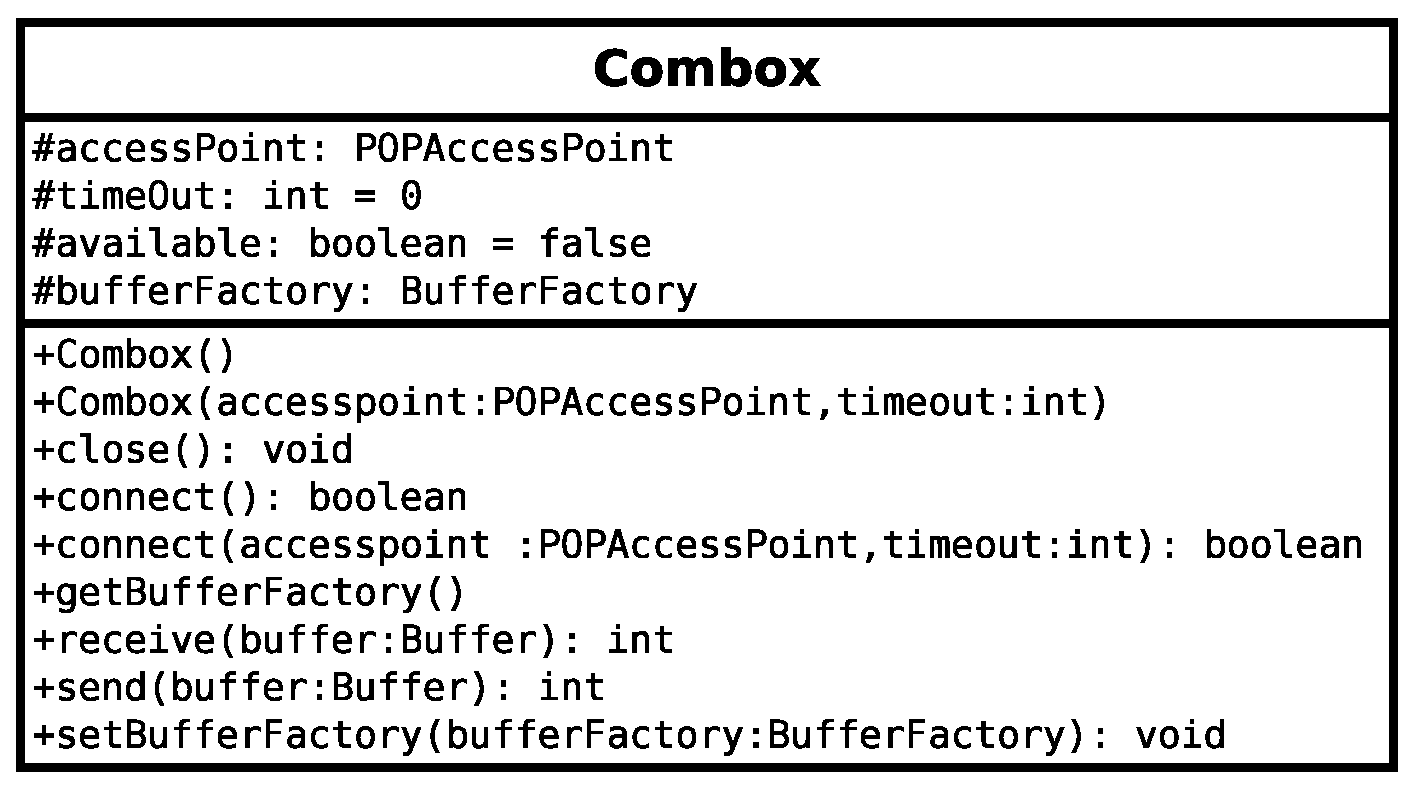
\includegraphics[scale=0.5]{combox.eps}
\end{figure}
\pagebreak

The combox server must inherits from the super class ComboxServer located in the package popjava.combox in the POP-Java library. The figure[\ref{fig:comboxserver_class}] shows the ComboxServer class signature. 

\begin{figure}[ht]
\caption{ComboxServer signature}
\center
\label{fig:comboxserver_class}
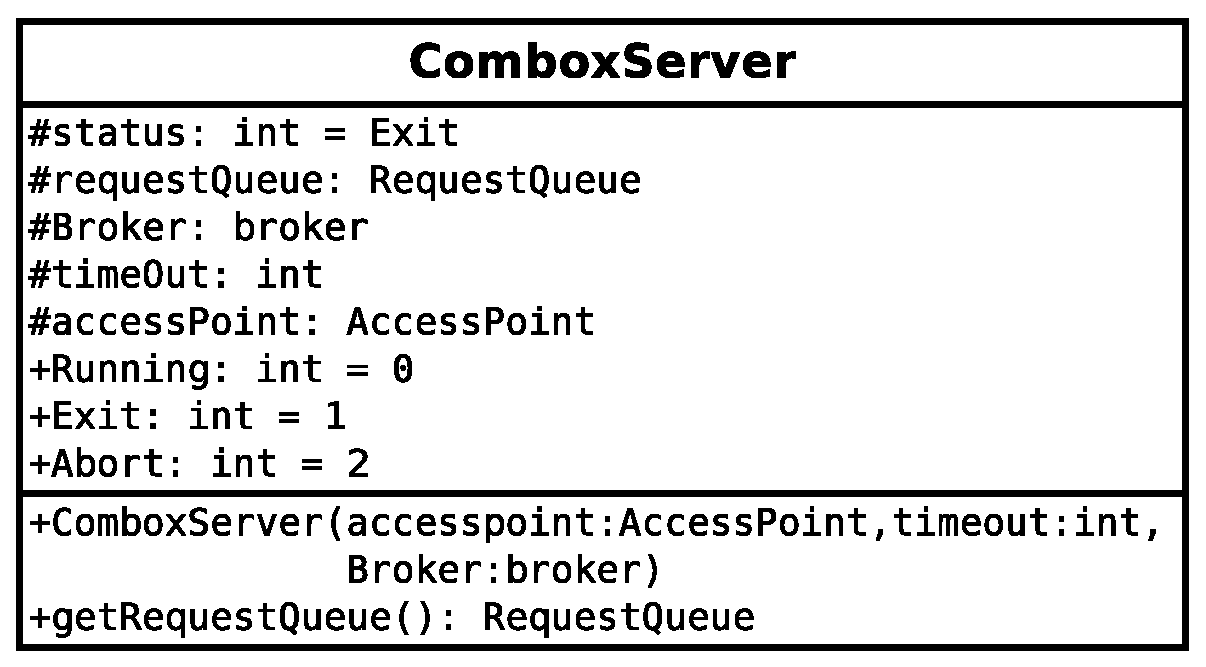
\includegraphics[scale=0.5]{comboxserver.eps}
\end{figure}

The combox factory must inherits from the super class ComboxFactory located in the package popjava.combox in the POP-Java library. The figure[\ref{fig:comboxfactory_class}] shows the ComboxFactory class signature.

\begin{figure}[ht]
\caption{ComboxFactory class signature}
\center
\label{fig:comboxfactory_class}
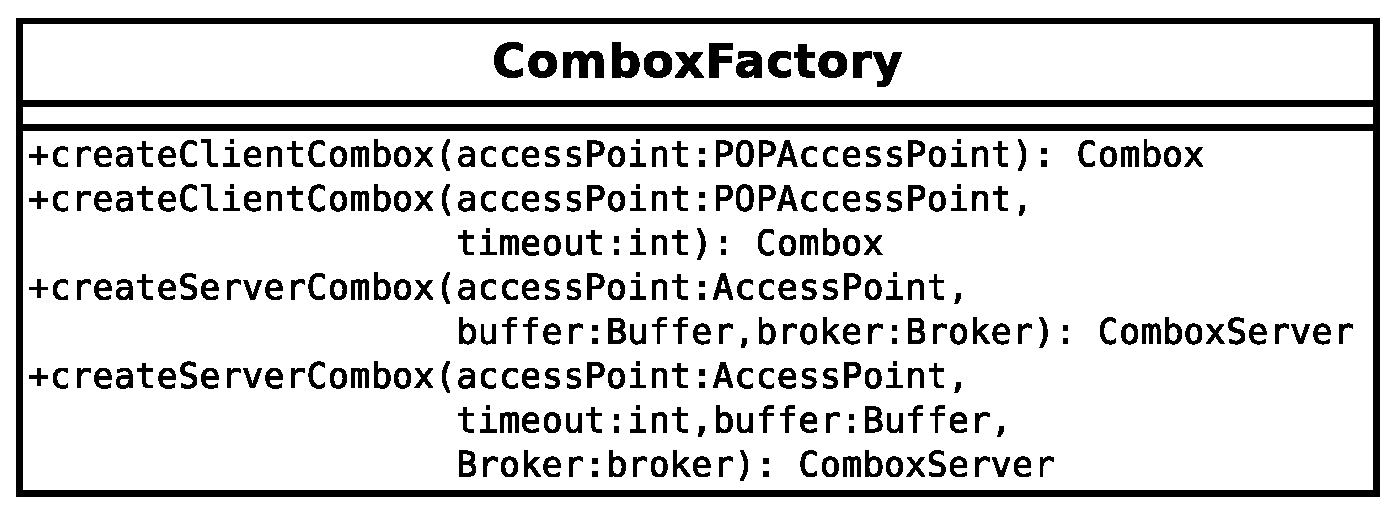
\includegraphics[scale=0.5]{comboxfactory.eps}
\end{figure}


Once all the classes are implemented, the programmer needs to compile them as standard Java code and create a JAR file. This JAR file can be added in the system by editing the file pop\_combox.xml located in the directory \textit{POPJAVA\_LOCATION/plugin}. The XML code below is the current XML file with the socket protocol.

\begin{lstlisting}
<ComboxFactoryList>
  <Package JarFile="popjava.combox.jar">
    <ComboxFactory>popjava.combox.ComboxSocketFactory</ComboxFactory>
  </Package>
</ComboxFactoryList>
\end{lstlisting}


\pagebreak
\subsection{Buffer plugin}
The buffer is the component in charge of the data encoding. In the current implementation of POP-Java, two buffers are available. One is using the RAW encoding and the other is using the XDR encoding. If the programmer needs a special encoding protocol, he can also create his own and add it to the POP-Java system as a plugin. \s

To implement a new encoding protocol, the programmer needs to create two class. A buffer and a buffer factory. \s

The buffer must inherits from the super class BufferPlugin located in the package popjava.buffer in the POP-Java library. The figure[\ref{fig:buffer_class}] shows the BufferPlugin class signature.
\begin{figure}[ht]
\caption{BufferPlugin class signature}
\center
\label{fig:buffer_class}
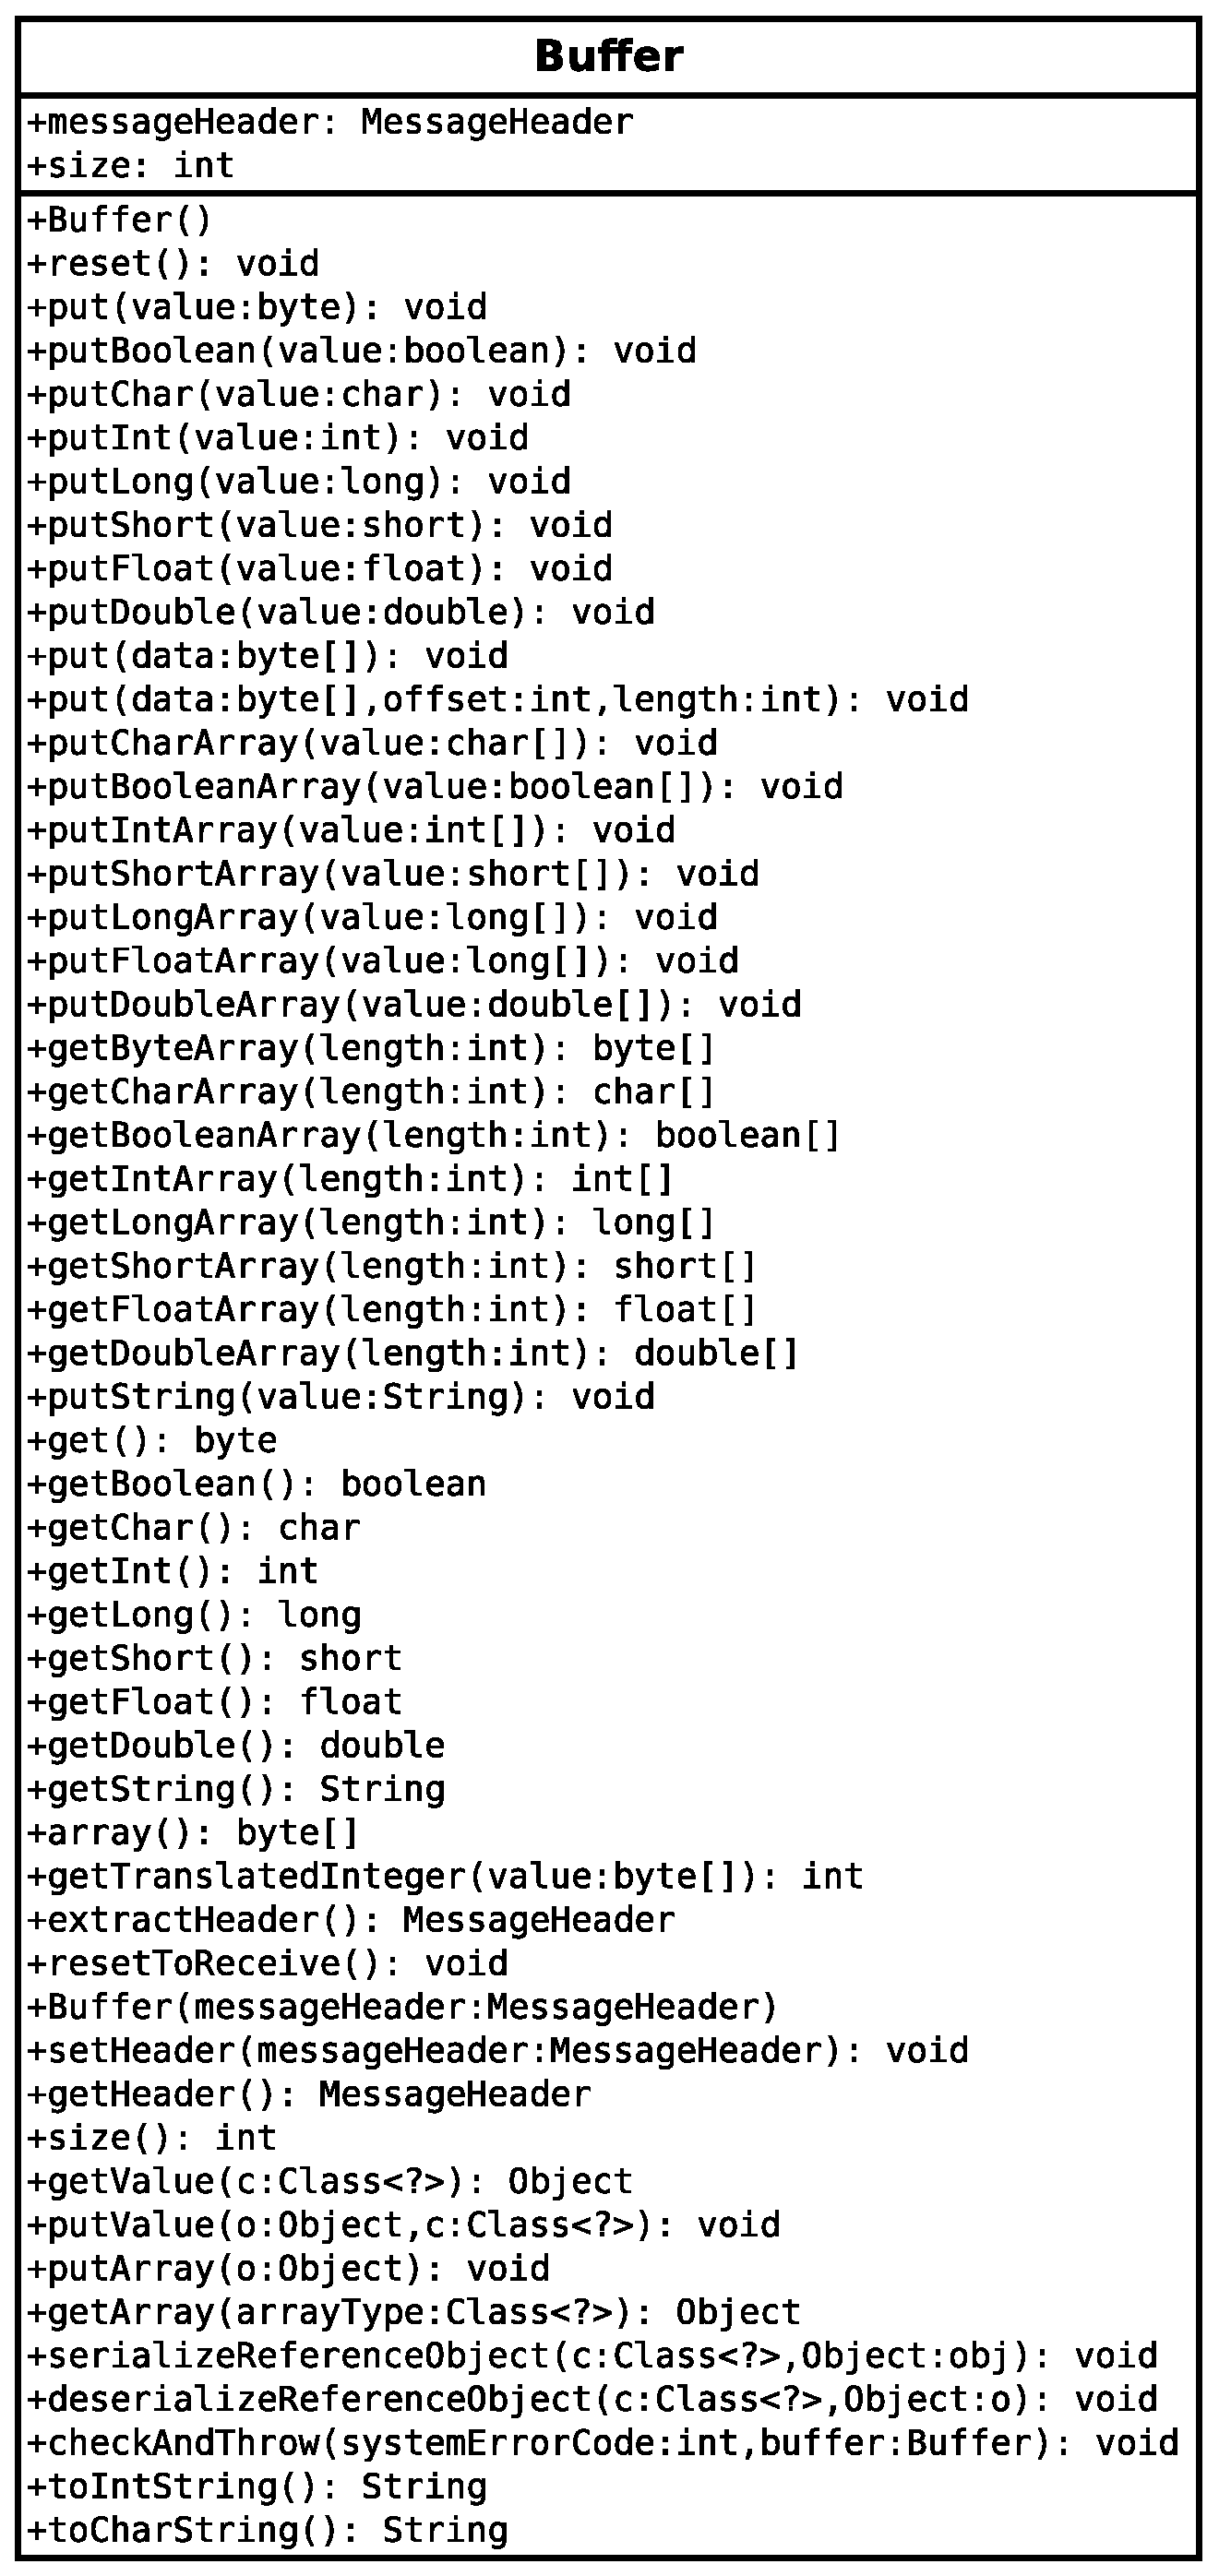
\includegraphics[scale=0.35]{buffer.eps}
\end{figure}

\pagebreak
The buffer factory must inherits from the super class BufferFactory located in the package popjava.buffer in the POP-Java library. The figure[\ref{fig:bufferfactory_class}] shows the BufferFactory class signature.
\begin{figure}[ht]
\caption{BufferFactory class signature}
\center
\label{fig:bufferfactory_class}
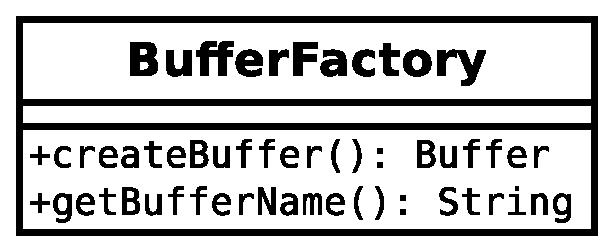
\includegraphics[scale=0.5]{bufferfactory.eps}
\end{figure}



% INSTALLATION
\pagebreak
\section{Installation}
\label{install}
To use POP-Java and POP-C++ on a computer we need to install them. This chapter helps the programmer to perform the correct installation of the POP system on a computer.

\subsection{POP-C++ installation}
In order to use POP-Java we need to install the latest version of POP-C++. This section will help us to get trough th installation process and make sure the installation is fine for a POP-Java usage.

\subsubsection{Requirements}
In order to install POP-C++ we need few additional software. The following packages are required before compiling : 
\begin{itemize}
\item a C++ compiler (g++ or equivalent)
\item zlib-devel (package name depends on distribution)
\item Gnu Bison (optional)
\item Globus Toolkit (optional)
\end{itemize}

\subsubsection{Before installing}
Before installation we should make the following configuration choices. In case of doubt the default values can be used.
\begin{itemize}
\item The compilation directory that should hold roughly 50MB. This directory will contain the distribution tree and the source files of POP-C++. It may be erased after installation.
\item The installation directory that will hold less than 40M. It will contain the compiled files for POP-C++, include and configuration files. This directory is necessary in every computer executing POP-C++ program (default location /usr/local/popc).
\item A temporary directory will be asked in the installation process. This directory will be used by POP-C++ to hold file during the application execution (default /tmp).
\item Resource topology. The administrator must choose what computer form the grid.
\end{itemize}

For more informations about the POP-C++ installation and configuration process, please see "Parallel Object Programming C++ - User and Installation Manual"\cite{popc_intro}.

\pagebreak
\subsubsection{Installation process}
This section will guide us trough the POP-C++ installation process. In the POP distribution we find a directory including POP-C++. First, we need to configure the installation. If we use the configure script without any option, POP-C++ will be installed in the default directory (/usr/local/popc). We can also specify the directory by using the option --prefix.\s

\textbf{Default directory}
\begin{lstlisting}
./configure
\end{lstlisting}\s

\textbf{Specific directory}
\begin{lstlisting}
./configure --prefix=/home/user/popc
\end{lstlisting}\s

Once the configuration script is done, we will need to compile the source of POP-C++ for our architecture. For this, we just need to run the make command in the root directory of POP-C++.
\begin{lstlisting}
make
\end{lstlisting}\s

Finally, to install POP-C++, we need to run the install target of the make file. This script will guide us trough the installation. To be sure that our installation will fit the requirements of POP-Java, please follow the instructions below.\s

Answer "y" to the first question. We need to configure POP-C++ services.
\begin{lstlisting}
make install
...
DO YOU WANT TO CONFIGURE POP-C++ SERVICES? (y/n)
y
\end{lstlisting}\s

We need to make a special installation so answer "n" to the second question.
\begin{lstlisting}
...
DO YOU WANT TO MAKE A SIMPLE INSTALLATION ? (y/n) : 
n
\end{lstlisting}\s

\pagebreak
The answers to the questions below are up to our configuration but if we don't know our configuration just pass every question.
\begin{lstlisting}
=====================================================
GENERATING SERVICE MAPS...
CONFIGURING POP-C++ SERVICES ON YOUR LOCAL MACHINE...
Enter the full qualified master host name (POPC gateway):

Enter the child node:

Enter number of processors available (default:1):

Enter the maximum number of POP-C++ jobs that can run concurrently 
(default: 100):

Enter the available RAM for job execution in MB (default 1024) :

Which local user you want to use for running POP-C++ jobs?

CONFIGURING THE RUNTIME ENVIRONMENT
Enter the script to submit jobs to the local system:

Communication pattern:

SETTING UP RUNTIME ENVIRONMENT VARIABLES
Enter variable name:

\end{lstlisting}\s

We need the startup script to use the global runtime service with POP-Java so answer "y" to the question "Do you want to generate the POP-C++ startup scripts?".
\begin{lstlisting}
=====================================================
CONFIGURATION POP-C++ SERVICES COMPLETED!
=====================================================
Do you want to generate the POP-C++ startup scripts? (y/n)
y
\end{lstlisting}\s

\pagebreak
Depends on our configuration, we can modify the default values of the startup script or just keep them. One important thing is to copy the environment variables on the .bashrc or equivalent file.
\begin{lstlisting}
=====================================================
CONFIGURING STARTUP SCRIPT FOR YOUR LOCAL MACHINE...
Enter the service port[2711]:

Enter the domain name:

Enter the temporary directory for intermediate results:

=====================================================
CONFIGURATION DONE!
=====================================================

IMPORTANT : Do not forget to add these lines to your .bashrc 
file or equivalent :
---------
    POPC_LOCATION=/home/clementval/popc
    PATH=\$PATH:\$POPC_LOCATION/bin:\$POPC_LOCATION/sbin

Press <Return> to continue
\end{lstlisting}\s



The POP-C++ installation is done. We can now use POP-C++ and also install POP-Java.

\subsubsection{System startup}
Before executing any POP-C++ application, the runtime system (Job manager and resource discovery) must be started. There is a script provided for that purpose, so every node must run the following command: 
\begin{lstlisting}
POPC_LOCATION/sbin/SXXpopc start
\end{lstlisting}\s

SXXpopc is a standard Unix deamon control script, with the traditional start, stop and restart options.


\pagebreak
\subsection{POP-Java installation}
This section will guide us trough the POP-Java installation process.

\subsubsection{Requirements}
In order to install POP-Java, some packages are required. Here is the list of required packages : 
\begin{itemize}
\item JDK 7 or higher
\item POP-C++ 2.5 or higher
\item JavaCC (optional)
\item Apache ANT (optional)
\end{itemize}

\subsubsection{Installation process}
To install POP-Java we need to launch the command \textbf{ant} int the POP-Java directory. Once the source code is compiled,
launch the installation with the install script: \textbf{sudo ./install}.
This script will guide us trough the installation by asking us some questions.
Be aware that if we install POP-Java in the default location we need the administrator rights.
Please use the option "-E" with the sudo command to keep the environment variables.\s

Here is the output we should have on our shell : \s

\begin{lstlisting}
[POP-Java installation]: Detecting java executable ...
[POP-Java installation]: Java executable detected under 
  /usr/bin/java
[POP-Java installation]: Please enter the location of your desired 
  POP-Java installation (default: /usr/local/popj ) : 
/home/clementval/popj
[POP-Java installation]: Installing POP-Java under 
  /home/clementval/popj ? (y/n)
y
[POP-Java installation]: Copying files ...
[POP-Java installation]: Generating configuration files ...
[POP-Java installation]: Generating object map file for the test suite
[POP-Java installation]: POP-Java has been installed under 
  /home/clementval/popj. Please copy the following lines into your 
  .bashrc files or equivalent

POPJAVA_LOCATION=/home/clementval/popj
export POPJAVA_LOCATION
POPJAVA_JAVA=/usr/bin/java
export POPJAVA_JAVA
PATH=$PATH:$POPJAVA_LOCATION/bin

[POP-Java installation]: Installation done.
\end{lstlisting}

At the end of the installation, the script ask us to copy some environment variable declarations in the .bashrc or equivalent file.
This step is mandatory to make POP-Java work correctly.

\subsection{Test the installation}
POP-Java includes a test suite. We can run this test suite to check if our POP system is correctly installed.
To run this test suite, we need to launch the "launch\_testsuite" script located in the POP-Java installation location.

Here is the output we should get after the completion of the test suite : 
\begin{lstlisting}[basicstyle=\ttfamily\scriptsize]
./launch_testsuite 
########################################
#   POP-Java 1.0 Test Suite started    #
########################################
POP-C++ detected under /home/clementval/popc
POP-C++ was not running. Starting POP-C++ runtime global services ...
Starting POPC Job manager service: 
POPCSearchNode access point: socket://172.28.10.67:38331
Starting Parallel Object JobMgr service 
socket://172.28.10.67:2711POP-C++ started
##############################
#   POP-Java standard test   #
##############################
Starting POP-Java test suite
Launching passing arguments test (test 1/6)... 
Arguments test successful
Passing arguments test is finished ... 
Launching multi parallel object test (test 2/6)... 
Multiobjet test started ...
Result is : 1234
Multiobjet test finished ...
Multi parallel object test is finished... 
Launching callback test (test 3/6)... 
Callback test started ...
Identity callback is -1
Callback test successful
Callback test is finished... 
Launching barrier test (test 4/6)... 
Barrier: Starting test...
Barrier test successful
Barrier test is finished... 
Launching integer test (test 5/6)... 
i1 = 23
i2 = 25
i1+i2 = 48
Test Integer Successful
Integer test is finished... 
Launching Demo POP-Java test (test 6/6)... 
START of DemoMain program with 4 objects
Demopop with ID=1 created with access point : socket://127.0.1.1:39556
Demopop with ID=2 created with access point : socket://127.0.1.1:60575
Demopop with ID=3 created with access point : socket://127.0.1.1:50088
Demopop with ID=4 created with access point : socket://127.0.1.1:39475
Demopop:1 with access point socket://127.0.1.1:39556 is sending his ID to object:2
Demopop:2 receiving id=1
Demopop:2 with access point socket://127.0.1.1:60575 is sending his ID to object:3
Demopop:3 receiving id=2
Demopop:3 with access point socket://127.0.1.1:50088 is sending his ID to object:4
Demopop:4 receiving id=3
Demopop:4 with access point socket://127.0.1.1:39475 is sending his ID to object:1
Demopop:1 receiving id=4
END of DemoMain program
Demo POP-Java test is finished... 

####################################
#   POP-C++ interoperability test  #
####################################
popcc -o main integer.ph integer.cc main.cc
popcc -object -o integer.obj integer.cc integer.ph main.cc
./integer.obj -listlong > obj.map
Launching POP-C++ integer with POP-Java application test (test 1/2)
POPC Integer test started ...
o1 = 10
o2 = 20
10 + 20 = 30
POPC Integer test successful
POP-C++ integer with POP-Java application test is finishied ...
popcc -parclass-nobroker -c integer2.ph
popcc -o main integer2.stub.o integer.ph integer.cc main.cc
popcc -parclass-nobroker -c integer2.ph
popcc -object -o integer.obj integer2.stub.o integer.cc integer.ph
popcc -object -o integer2.obj integer2.cc integer2.ph
./integer.obj -listlong > obj.map
./integer2.obj -listlong >> obj.map
Launching Integer mix (POP-C++ and POP-Java) with POP-Java application test(test 2/2)
i=20
j=12
i+j=32
Integer mix (POP-C++ and POP-Java) with POP-Java application test is finishied ...
########################################
#   POP-Java 1.0 Test Suite finished   #
########################################
Stopping POPC Job manager service...
Connecting to 172.28.10.67:2711....
POPCSearchNode stopped
JobMgr stopped
\end{lstlisting}


%DOCUMENTATION AND EXAMPLE
%\emptypage
\pagebreak
\section{Documentation and examples}
\subsection{Documentation}
All the library is documented under the Javadoc format. This documentation is installed on the computer after the completion of the POP-Java installation. A generated documentation under the standard Javadoc and also under the Doxygen format is available. The "index.html" file is located in the folder \textit{POPJAVA\_LOCATION}/doc/index.html gives acces to both Javadoc and Doxygen documentation.

\subsection{Examples}
The POP-Java distribution includes some examples of POP-Java application. These examples can be found in the folder \textit{POPJAVA\_DISTRIBUTION}/example. All examples have a makefile to compile and a special target "run" to run these examples. The following examples are available for the moment : 

\begin{itemize}
\item Callback example : this example shows the ability of a parallel object to call back the one who called him.
\item Integer example : this is a simple example of a parallel object integer (same as the example in POP-C++).
\item Mixed1 example : this example is a POP-Java application using a POP-C++ integer parallel object
\item Mixed2 example : this example is a POP-C++ application using a POP-Java integer parallel object.
\item Multiobj example : this example shows a chaining of parallel object.
\end{itemize}


% TROURBLESHOOTING
%\emptypage
\pagebreak
\section{Troubleshooting}
\label{trouble}

\subsection{POP-Java exception}
This section lists some of the main POP-Java exception that can occurred during the application execution and gives the cause of the problem.

\subsubsection{Cannot bind to access point : socket://your-computer-name:2711}
This exception occurred when the application cannot contact the POP-C++ runtime system. To fix this problem, we need to start the POP-C++ runtime system with the following command : 

\begin{lstlisting}
POPC_LOCATION/sbin/SXXpopc start
\end{lstlisting}

\subsubsection{Error message : OBJECT\_EXECUTABLE\_NOTFOUND}
This exception occurred when the executable file is not found. This might be due to a bad object map or the deletion of the object executable file. To fix this problem we should generate a new object map with the object executable.

\subsubsection{Error message : NO\_RESOURCE\_MATCH}
This exception occurred when no resource match the requirements of a specific object. To fix this problem we should check the object descriptions in the parallel objects. We might have put a too high requirements for a parallel object creation.

\subsubsection{Error message : Cannot run program "/usr/local/popc/services/appservice"}
If we get an error with "cannot run program" and the path contains the appservice of POP-C++, sou have certainly reinstalled POP-C++ and the configuration file of POP-Java is now wrong. The easiest way to fix this problem is to reinstall also POP-Java. We can also edit the configuration file under \textit{POPJAVA\_LOCATION}/etc/popj\_config.xml. The item \textbf{popc\_appcoreservice\_location} must be modified with the good path.

\subsubsection{Test suite frozen}
If the test suite seems to be frozen, we should abort the test suite and restart the POP-C++ global service with the following command
\begin{lstlisting}
POPC_LOCATION/sbin/SXXpopc restart
\end{lstlisting}


%\emptypage
\pagebreak
\section{Table of figures}
\listoffigures{}


%\emptypage
\pagebreak
\section{References}
\begin{thebibliography}{9}

\bibitem{popjava_tech}
	Clément Valentin,
  	\emph{POP-Java - Technical Report}.
	EIA-FR, Fribourg, Switzerland,
	August 2010.

\bibitem{popc_intro}
	The POP-C++ Team,
  	\emph{Parallel Object Programming C++, User and installation Manual}.
	Grid and Ubiquitous Computing Group, EIA-FR, Fribourg, Switzerland,
	2010.

\bibitem{popc_thesis}
	Dr. Thuan-Anh Nguyen,
  	\emph{An object-oriented model for adaptive high performance computing on the computational GRID}.
	EPFL, Lausanne, Switzerland,
	2005.

\bibitem{Allcock02}
W.~Allcock, J.~Bester, J.~Bresnahan, A.~Chervenak, L.~Liming, S.~Meder, and
  S.~Tuecke.
\newblock {\em GridFTP Protocol Specification}.
\newblock GGF GridFTP Working Group Document, September 2002.
\newblock http://www.globus.org/research/papers.htm.

\bibitem{Czajkowski98}
K.~Czajkowski, I.~Foster, N.~Karonis, C.~Kesselman, S.~Martin, W.~Smith, and
  S.~Tuecke.
\newblock A resource management architecture for metacomputing systems.
\newblock In {\em Proc. IPPS/SPDP '98 Workshop on Job Scheduling Strategies for
  Parallel Processing}, pages 62--82, 1998.

\bibitem{Foster98:2}
I.~Foster and N.~Karonis.
\newblock A grid-enabled mpi: Message passing in heterogeneous distributed
  computing systems.
\newblock In {\em Proc. 1998 SC Conference}, November 1998.

\bibitem{Foster97}
I.~Foster and C.~Kesselman.
\newblock Globus: A metacomputing infrastructure toolkit.
\newblock {\em Intl J. Supercomputer Applications}, 11(2):115--128, 1997.

\bibitem{Foster02}
I.~Foster, C.~Kesselman, J.~Nick, and S.~Tuecke.
\newblock Grid services for distributed system integration.
\newblock {\em Computer}, 35(6), 2002.

\bibitem{Grimshaw99}
Andrew Grimshaw, Adam Ferrari, Fritz Knabe, and Marty Humphrey.
\newblock Legion: An operating system for wide-area computing.
\newblock {\em IEEE Computer}, 32:5:29--37, May 1999.

\bibitem{Karonis03}
N.~Karonis, B.~Toonen, and I.~Foster.
\newblock {MPICH-G2}: A grid-enabled implementation of the message passing
  interface.
\newblock {\em Journal of Parallel and Distributed Computing}, 2003.

\bibitem{Nguyen07}
Kuonen~P. Nguyen, T.~A.
\newblock Programming the grid with pop-c++.
\newblock {\em Future Generation Computer Systems (FGCS)}, 23(1):23--30,
  January 2007.

\bibitem{Nguyen04}
Tuan-Anh Nguyen.
\newblock {\em An Object-oriented model for adaptive high performance computing
  on the computational Grid}.
\newblock PhD thesis, Swiss Federal Institute of Technology-Lausanne, 2004.

\bibitem{corba26}
{Object Management Group}, Framingham, Massachusetts.
\newblock {\em The Common Object Request Broker: Architecture and Specification
  --- Version 2.6}, December 2001.

\bibitem{Roy00}
A.~Roy, I.~Foster, W.~Gropp, N.~Karonis, V.~Sander, and B.~Toonen.
\newblock \mbox{MPICH-GQ}: Quality-of-service for message passing programs.
\newblock In {\em Proc. of the IEEE/ACM SC2000 Conference}, November 2000.

\bibitem{Stockinger01}
H.~Stockinger, A.~Samar, B.~Allcock, I.~Foster, K.~Holtman, and B.~Tierney.
\newblock File and object replication in data grids.
\newblock In {\em 10th IEEE Symposium on High Performance and Distributed
  Computing (HPDC2001)}, 2001.
\newblock San Francisco, California.

\bibitem{Tong03}
Weiqin Tong, Jingbo Ding, and Lizhi Cai.
\newblock A parallel programming environment on grid.
\newblock In {\em International Conference on Computational Science 2003},
  pages 225--234, 2003.

\bibitem{Welch03}
V.~Welch, F.~Siebenlist, I.~Foster, J.~Bresnahan, K.~Czajkowski, J.~Gawor,
  C.~Kesselman, S.~Meder, L.~Pearlman, and S.~Tuecke.
\newblock Security for grid services.
\newblock In IEEE Press, editor, {\em Twelfth International Symposium on High
  Performance Distributed Computing (HPDC-12)}, 2003.

\bibitem{Williams00}
Tiffani~L. Williams and Rebecca~J. Parsons.
\newblock The heterogeneous bulk synchronous parallel model.
\newblock {\em Lecture Notes in Computer Science}, 1800, 2000.

\end{thebibliography}

\pagebreak
\appendix
\section{POP-Java compiler command}
\label{popjc_help}
\begin{lstlisting}
POP-Java Compiler v1.0

This program is used to compile a POP-Java program

Usage: popjc <options> <source files>

OPTIONS:
   -h, --help               Show this message
   -n, --noclean            Do not clean the intermediate Java file 
                            generated by the POP-Java parser
   -p, --popcpp <xml_file>  Compile a POP-Java parallel class for 
                            POP-C++ usage (Need XML additional 
                            informations file)
   -j, --jar <filename>     Create a JAR archive with the given name 
                            (Need the JAR file name)       
   -v, --verbose            Verbose mode
   -c, --classpath <files>  Include JAR or compiled Java class to the 
                            compilation process. Files must be 
                            separated by a semicolon ":"

OPTIONS FOR POP-C++ INTEROPERABILITY:
   -x, --xmlpopcpp <files>  Generate a canvas of the POP-C++ XML 
                            additional informations file for the 
                            given Java files. This option must be 
                            used alone.
   -g, --generate <pjava>   Generate the POP-C++ partial 
                            implementation to use the given 
                            POP-Java parclass in a POP-C++ application 
                            (NOT IMPLEMENTED YET)
\end{lstlisting}

%\emptypage
\pagebreak
\section{POP-Java application launcher command}
\begin{lstlisting}
POP-Java Application Runner v1.0

This program is used to run a POP-Java application or to generate 
object map

Usage: popjrun <options> <objectmap> <mainclass>

OPTIONS:
   -h, --help                Show this message
   -v, --verbose             Verbose mode
   -c, --classpath <files>   Include JAR or compiled Java class 
                             needed to run the application. Files must 
                             be separated by a semicolon ":"

OPTIONS FOR OBJECT MAP GENERATION:
   -l, --listlong <parclass> Generate the object map for the given 
                             parclasses. Parclasses can be a .class, 
                             .jar, .obj or .module file. Parclasses 
                             must be separated by : 


\end{lstlisting}



\end{document}
